% XeLaTeX can use any Mac OS X font. See the setromanfont command below.
% Input to XeLaTeX is full Unicode, so Unicode characters can be typed directly into the source.

% The next lines tell TeXShop to typeset with xelatex, and to open and save the source with Unicode encoding.

%!TEX TS-program = xelatex
%!TEX encoding = UTF-8 Unicode

\documentclass[11pt,twoside,openany]{book}
\usepackage{multirow}
\usepackage{pdfpages}
\usepackage{xspace}
\usepackage{array}
\usepackage{lipsum}

\usepackage{algorithm}
\usepackage{algpseudocode}

\usepackage{geometry}                % See geometry.pdf to learn the layout options. There are lots.
%\usepackage[margin=1cm]{geometry}


%	\addtolength{\textwidth}{1.75in}
%
%	\addtolength{\topmargin}{-.875in}
%	\addtolength{\textheight}{1.75in}

\geometry{a4paper,left=20mm,top=20mm,bottom=50mm,total={162mm,230mm}}                   % ... or a4paper or a5paper or ...
%\geometry{landscape}                % Activate for for rotated page geometry
%\usepackage[parfill]{parskip}    % Activate to begin paragraphs with an empty line rather than an indent
\usepackage{amssymb}
%\usepackage{todonotes}
\setlength{\marginparwidth}{2cm}
\usepackage[backgroundcolor=white,bordercolor=blue,linecolor=blue,textwidth=1cm]{todonotes}
\usepackage{booktabs}
\usepackage{longtable}
\usepackage{url}

\usepackage[depth=4]{bookmark}


\usepackage{algorithm}
\usepackage{algpseudocode}

\usepackage{imakeidx}
\usepackage[utf8]{inputenc}
\usepackage[T1]{fontenc}
\makeindex[intoc]

\usepackage[font=normalsize]{caption}

\usepackage{hyperref}
\hypersetup{
    colorlinks,
    citecolor=black,
    filecolor=black,
    linkcolor=black,
    urlcolor=black
}

\renewcommand{\theparagraph}{\S\arabic{paragraph}}
\setcounter{secnumdepth}{4}


\usepackage{xcolor}
\usepackage{listings}

\makeatletter
\global\let\tikz@ensure@dollar@catcode=\relax
\makeatother

\definecolor{mGreen}{rgb}{0,0.6,0}
\definecolor{mGray}{rgb}{0.5,0.5,0.5}
\definecolor{mPurple}{rgb}{0.58,0,0.82}
\definecolor{backgroundColour}{rgb}{0.95,0.95,0.92}
\definecolor{gray}{rgb}{0.4,0.4,0.4}
\definecolor{darkblue}{rgb}{0.0,0.0,0.6}
\definecolor{cyan}{rgb}{0.0,0.6,0.6}

\lstdefinestyle{CStyle}{
    backgroundcolor=\color{backgroundColour},
    commentstyle=\color{mGreen},
    keywordstyle=\color{magenta},
    numberstyle=\tiny\color{mGray},
    stringstyle=\color{mPurple},
    basicstyle=\scriptsize\ttfamily,
    breakatwhitespace=false,
    breaklines=true,
    captionpos=b,
    keepspaces=true,
    numbers=left,
    numbersep=5pt,
    showspaces=false,
    showstringspaces=false,
    showtabs=false,
    tabsize=2,
    language=C
}


\lstset{
  backgroundcolor=\color{white},   % choose the background color; you must add \usepackage{color} or \usepackage{xcolor}; should come as last argument
  basicstyle=\footnotesize\ttfamily,        % the size of the fonts that are used for the code
  breakatwhitespace=false,         % sets if automatic breaks should only happen at whitespace
  breaklines=true,                 % sets automatic line breaking
  captionpos=b,                    % sets the caption-position to bottom
  commentstyle=\color{gray},    % comment style
  deletekeywords={...},            % if you want to delete keywords from the given language
  %escapeinside={\%*}{*)},          % if you want to add LaTeX within your code
  %extendedchars=true,              % lets you use non-ASCII characters; for 8-bits encodings only, does not work with UTF-8
  %firstnumber=1000,                % start line enumeration with line 1000
  frame=single,	                   % adds a frame around the code
  keepspaces=true,                 % keeps spaces in text, useful for keeping indentation of code (possibly needs columns=flexible)
  keywordstyle=\color{blue},       % keyword style
  language=C,                 % the language of the code
  %morekeywords={*,...},            % if you want to add more keywords to the set
  numbers=left,                    % where to put the line-numbers; possible values are (none, left, right)
  numbersep=5pt,                   % how far the line-numbers are from the code
  numberstyle=\tiny\color{gray}, % the style that is used for the line-numbers
  rulecolor=\color{black},         % if not set, the frame-color may be changed on line-breaks within not-black text (e.g. comments (green here))
  showspaces=false,                % show spaces everywhere adding particular underscores; it overrides 'showstringspaces'
  showstringspaces=false,          % underline spaces within strings only
  showtabs=false,                  % show tabs within strings adding particular underscores
  stepnumber=1,                    % the step between two line-numbers. If it's 1, each line will be numbered
  stringstyle=\color{black},     % string literal style
  tabsize=2,	                   % sets default tabsize to 2 spaces
}

\lstset{
  columns=fullflexible,
  showstringspaces=false,
  commentstyle=\color{gray}\upshape,
  backgroundcolor=\color{backgroundColour},
  commentstyle=\color{mGreen},
  keywordstyle=\color{magenta},
  numberstyle=\tiny\color{mGray},
  stringstyle=\color{mPurple},
  basicstyle=\scriptsize\ttfamily,
  tabsize=2
}

\lstdefinelanguage{XML}
{
  morestring=[b]",
  morestring=[s]{>}{<},
  morecomment=[s]{<?}{?>},
  stringstyle=\color{black},
  identifierstyle=\color{darkblue},
  keywordstyle=\color{cyan},
  morekeywords={xmlns,version,type}% list your attributes here
}


% Will Robertson's fontspec.sty can be used to simplify font choices.
% To experiment, open /Applications/Font Book to examine the fonts provided on Mac OS X,
% and change "Hoefler Text" to any of these choices.

\usepackage{fontspec,xltxtra,xunicode}
\defaultfontfeatures{Mapping=tex-text}
\setromanfont[Mapping=tex-text]{Optima}
\setsansfont[Scale=MatchLowercase,Mapping=tex-text]{Optima}
\setmonofont[Scale=MatchLowercase]{Andale Mono}

%%%% Graphics
\usepackage{graphicx}
\usepackage{tikz}
\definecolor{unilublue}{RGB}{55,149,218}
\definecolor{sntred}{RGB}{219,46,27}
\definecolor{sntpurple}{RGB}{86,30,130}
%\definecolor{sntblue}{RGB}{50,130,207}
\definecolor{sntblue}{RGB}{55,149,218}

\pgfdeclareimage[width=30mm]{logo-snt}{logos/logo-snt}
\pgfdeclareimage[width=30mm]{logo-uni-lu}{logos/logo-uni-lu}

%%%% Fancy
\usepackage{fancyhdr}

%%%% Increase page length
\addtolength{\textheight}{1in}

%%%% Sections
\usepackage{sectsty}
\allsectionsfont{\sffamily}

\setlength{\parskip}{1em}

%\renewcommand{\,}{$^{\cdot}$}

%%%% Title
\newcommand{\titleone}{\textsf{FAQAS Framework}}
\newcommand{\titletwo}{\textsf{SDD - Software Design Document}}
\newcommand{\titlethree}{\textsf{Software User Manual}}

\newcommand{\todoinline}[1]{\todo[color=orange,inline]{ \textbf{TODO}: #1 }}

\newcommand{\TODO}[1]{\todo[color=orange,inline]{ \textbf{TODO}: #1 }}
\newcommand{\OSCAR}[1]{\todo[color=yellow,inline]{ \textbf{OSCAR}: #1 }}
\newcommand{\DONE}[1]{\todo[color=green,inline]{ \textbf{DONE}: #1 }}

\newcommand{\CHANGEDTWO}[1]{\textcolor{black}{#1}}

\newcommand{\EMPH}[1]{\textbf{\emph{#1}}}
\newcommand{\INDEX}[1]{\index{\MakeLowercase{#1}}\EMPH{#1}}

\newcommand{\MASS}{\textit{MASS}\xspace}
\newcommand{\dama}{\textit{DaMAT}\xspace}

\newcommand{\STARTCHANGEDWPT}{\color{blue}}
\newcommand{\ENDCHANGEDWPT}{\color{black}}

\newcounter{paranum}
\newcommand{\RQ}{\vspace{10pt}\noindent\textbf{FAQAS-SSS-REQ-\refstepcounter{paranum}\ifnum\value{paranum}<10 00\else 0\fi\theparanum}\textbf}

\newcommand{\remark}{\textbf{Remark:}\xspace}


\begin{document}

\pagestyle{fancy}
\renewcommand{\sectionmark}[1]{\markright{\textit{#1}}}

\renewcommand{\headrulewidth}{2pt}% 2pt header rule
\renewcommand{\headrule}{\hbox to\headwidth{%
  \color{sntblue}\leaders\hrule height \headrulewidth\hfill}}

\fancyhf{}

%\lhead{\fancyplain{}{\setlength{\unitlength}{1mm}
%\begin{picture}(0,0)
%\put(0,-4){
\includegraphics[width=50pt]{logos/logo-snt}}
%\end{picture}}}

\newcommand{\DOCUMENTID}{ITT-1-9873-ESA-FAQAS-SDD}
\lhead{\fancyplain{}{\textit{\DOCUMENTID}}}
\rhead{\fancyplain{}{\rightmark }}


\fancyfoot[C]{%
\begin{tikzpicture}[remember picture,overlay]
\path [fill=sntred]    ([xshift=88pt,yshift=20pt]current page.south west) rectangle
                       ([xshift=229pt,yshift=50pt] current page.south west);
\path [fill=sntpurple] ([xshift=229pt,yshift=20pt] current page.south west) rectangle
                       ([xshift=370pt,yshift=50pt] current page.south west);
\path [fill=sntblue]   ([xshift=370pt,yshift=20pt] current page.south west) rectangle
                       ([xshift=510pt,yshift=50pt] current page.south west);
\end{tikzpicture}
}

\fancyfoot[RO]{
\begin{tikzpicture}[remember picture,overlay]
\node [circle, ultra thick, fill=white, draw=sntblue] at ([xshift=530pt,yshift=35pt] current page.south west) {\thepage};
\end{tikzpicture}}

\fancyfoot[LE]{
\begin{tikzpicture}[remember picture,overlay]
\node [circle, ultra thick, fill=white, draw=sntblue] at ([xshift=65pt,yshift=35pt] current page.south west) {\thepage};
\end{tikzpicture}}


\newcommand{\CHANGED}[1]{\textcolor{blue}{#1}}
\newcommand{\prog}{P}
\newcommand{\prop}{}

\newcommand{\stt}[1]{\begin{footnotesize}\texttt{{#1}}\end{footnotesize}}


\newcommand{\REVISION}[2]{{#2}}
%\newcommand{\REVISION}[2]{#2}

% \newcommand{\REVTWO}[2]{\todo[color=red]{\tiny{#1}}\textcolor{red}{#2}}
% \newcommand{\REVTWO}[2]{#2}
\newcommand{\FAQAS}{FAQAS-framework\xspace}

\thispagestyle{empty}

\begin{tikzpicture}[remember picture,overlay]
\path [fill=sntred]    ([xshift=30pt,yshift=20pt]current page.south west) rectangle
                       ([xshift=210pt,yshift=50pt] current page.south west);
\path [fill=sntpurple] ([xshift=210pt,yshift=20pt] current page.south west) rectangle
                       ([xshift=390pt,yshift=50pt] current page.south west);
\path [fill=sntblue]   ([xshift=390pt,yshift=20pt] current page.south west) rectangle
                       ([xshift=570pt,yshift=51pt] current page.south west);
\path [fill=unilublue] ([xshift=30pt,yshift= 50pt] current page.south west) --
                       ([xshift=570pt,yshift= 50pt] current page.south west)
                       [rounded corners=20pt] --
                       ([xshift=570pt,yshift=740pt] current page.south west)
                       [sharp corners] --
                       ([xshift=30pt,yshift=740pt] current page.south west);
\node [fill=white,rounded corners=0pt,inner xsep=6pt,inner ysep=3pt]
      at ([xshift=523pt,yshift=120pt] current page.south west)
      {\pgfuseimage{logo-uni-lu}};

\node [fill=white,rounded corners=2pt,inner xsep=6pt,inner ysep=3pt]
      at ([xshift=520pt,yshift=780pt] current page.south west)
      {\pgfuseimage{logo-snt}};

%\node [circle, fill=white, draw=sntblue] at ([xshift=550pt,yshift=35pt] current page.south west) {a};

\node[draw=none,fill=none,right] at (-1, -7){\color{white}\LARGE\bf\titleone};
\node[draw=none,fill=none,right] at (-1, -8){\color{white}\LARGE\bf\titletwo};
\node[draw=none,fill=none,right] at (-1, -9){\color{white}\LARGE\bf\titlethree};

\node[draw=none,fill=none,right] at (-1, -12){\color{white}\Large\textsf{O. Cornejo, F. Pastore, E. Viganò}};
\node[draw=none,fill=none,right] at (-1, -13){\color{white}\Large\textsf{Interdisciplinary Centre for Security, Reliability and Trust}};
\node[draw=none,fill=none,right] at (-1, -14){\color{white}\Large\textsf{University of Luxembourg}};
\node[draw=none,fill=none,right] at (11, -16){\color{white}\textsf{ITT-1-9873-ESA-FAQAS-SUTP}};
\node[draw=none,fill=none,right] at (11, -17){\color{white}\Large\textsf{Issue 4, Rev. 1}};
\node[draw=none,fill=none,right] at (11, -18){\color{white}\Large\textsf{\today}};
\node[draw=none,fill=none,right] at (-1, -24){\color{white}\tiny\textsf{EUROPEAN SPACE AGENCY. CONTRACT REPORT.}};
\node[draw=none,fill=none,right] at (-1, -24.3){\color{white}\tiny\textsf{The work described in this report was done under ESA contract. Responsibility for the contents resides in the author or organisation that prepared it.}};
\node[draw=none,fill=none,right] at (-1, -24.8){\color{white}\tiny\textsf{The copyright in this document is vested in the University of Luxembourg.}};
\node[draw=none,fill=none,right] at (-1, -25.1){\color{white}\tiny\textsf{This document may only be reproduced in whole or in part, or stored in a retrieval system,or transmitted in any form, or by any means electronic,}};
\node[draw=none,fill=none,right] at (-1, -25.4){\color{white}\tiny\textsf{mechanical, photocopying or otherwise, either with the prior permission of the University of Luxembourg or in accordance with the terms of ESTEC Contract No. 4000128969/19/NL/AS.}};

\node[draw=none,fill=none,right] at (-1, -24){\color{white}\tiny\textsf{EUROPEAN SPACE AGENCY. CONTRACT REPORT.}}; 
\node[draw=none,fill=none,right] at (-1, -24.3){\color{white}\tiny\textsf{The work described in this report was done under ESA contract. Responsibility for the contents resides in the author or organisation that prepared it.}};
\node[draw=none,fill=none,right] at (-1, -24.8){\color{white}\tiny\textsf{The copyright in this document is vested in the University of Luxembourg.}};
\node[draw=none,fill=none,right] at (-1, -25.1){\color{white}\tiny\textsf{This document may only be reproduced in whole or in part, or stored in a retrieval system,or transmitted in any form, or by any means electronic,}}; 
\node[draw=none,fill=none,right] at (-1, -25.4){\color{white}\tiny\textsf{mechanical, photocopying or otherwise, either with the prior permission of the University of Luxembourg or in accordance with the terms of ESTEC Contract No. 4000128969/19/NL/AS.}};


\end{tikzpicture}

\newpage


% !TEX root = MAIN.tex

\section*{Revisions}
\label{sec:revisions}


\setlength\LTleft{0pt}
\setlength\LTright{0pt}
\tiny 
%@{\extracolsep{\fill}}
\begin{longtable}{|p{2cm}|p{1cm}|p{1.5cm}|p{9cm}|@{}}
\label{table:codeoperators} \\
\hline
\textbf{Issue Number}&\textbf{Date}&\textbf{Authors}&\textbf{Description}\\
\hline
ITT-1-9873-ESA-FAQAS-FR
Issue 1 Rev. 1&
October 29th, 2021&
Fabrizio Pastore, Oscar Cornejo, Enrico Viganò&
\begin{minipage}{8cm}
Initial release.
\end{minipage}
\\
\hline
ITT-1-9873-ESA-FAQAS-FR
Issue 1 Rev. 2&
November 11th, 2021&
Fabrizio Pastore, Oscar Cornejo, Enrico Viganò&
\begin{minipage}{8cm}
Added Chapter~\ref{chap:deliverables_summary} (deliverables summary).\\
Added Chapter~\ref{ch:toolset} (description of toolset package).\\
Added information about input and outputs of the tools in Chapter~\ref{chapter:methodology} (see blue text).
\end{minipage}
\\
\hline
                                                    
\end{longtable}
\normalsize

\clearpage




\tableofcontents

% !TEX root = MAIN.tex

\chapter{Scope and content}

This document is the deliverable SSS of the ESA activity ITT-1-9873-ESA. It concerns requirements specification for the \emph{FAQAS framework} to be delivered by ITT-1-9873-ESA. Following the structure described in the SoW \emph{AO9873-ws00pe\_SOW.pdf}, it provides the structured requirements baseline for the FAQAS framework according to ECSS-E-ST-40C Annex B.
 
\section{Applicable and reference documents}

\begin{itemize}
\item{D1 - Mutation testing survey}
\item{D2 - Study of mutation testing applicability to space software}
\end{itemize}

\chapter{Terms, definitions and abbreviated terms}

\begin{itemize}
\item{FAQAS}: activity ITT-1-9873-ESA
\item{FAQAS-framework}: software system to be released at the end of WP4 of FAQAS
\item{D2}: Deliverable D2 of FAQAS, \emph{Study of mutation testing applicability to space software}
\item{KLEE}: Third party test generation tool, details are provided in D2.
\item{SUT}: Software under test, i.e, the software that should be mutated by means of mutation testing.
\item{WP}: Work package
\end{itemize}

\clearpage
 



% !TEX root = MAIN.tex

\chapter{Software Release Overview}

\chapter{Status of the Software Configuration Item}

\clearpage
% !TEX root = MAIN.tex

\section{MASS}

\subsection{Software static architecture}





\begin{figure}[h]
  \centering
	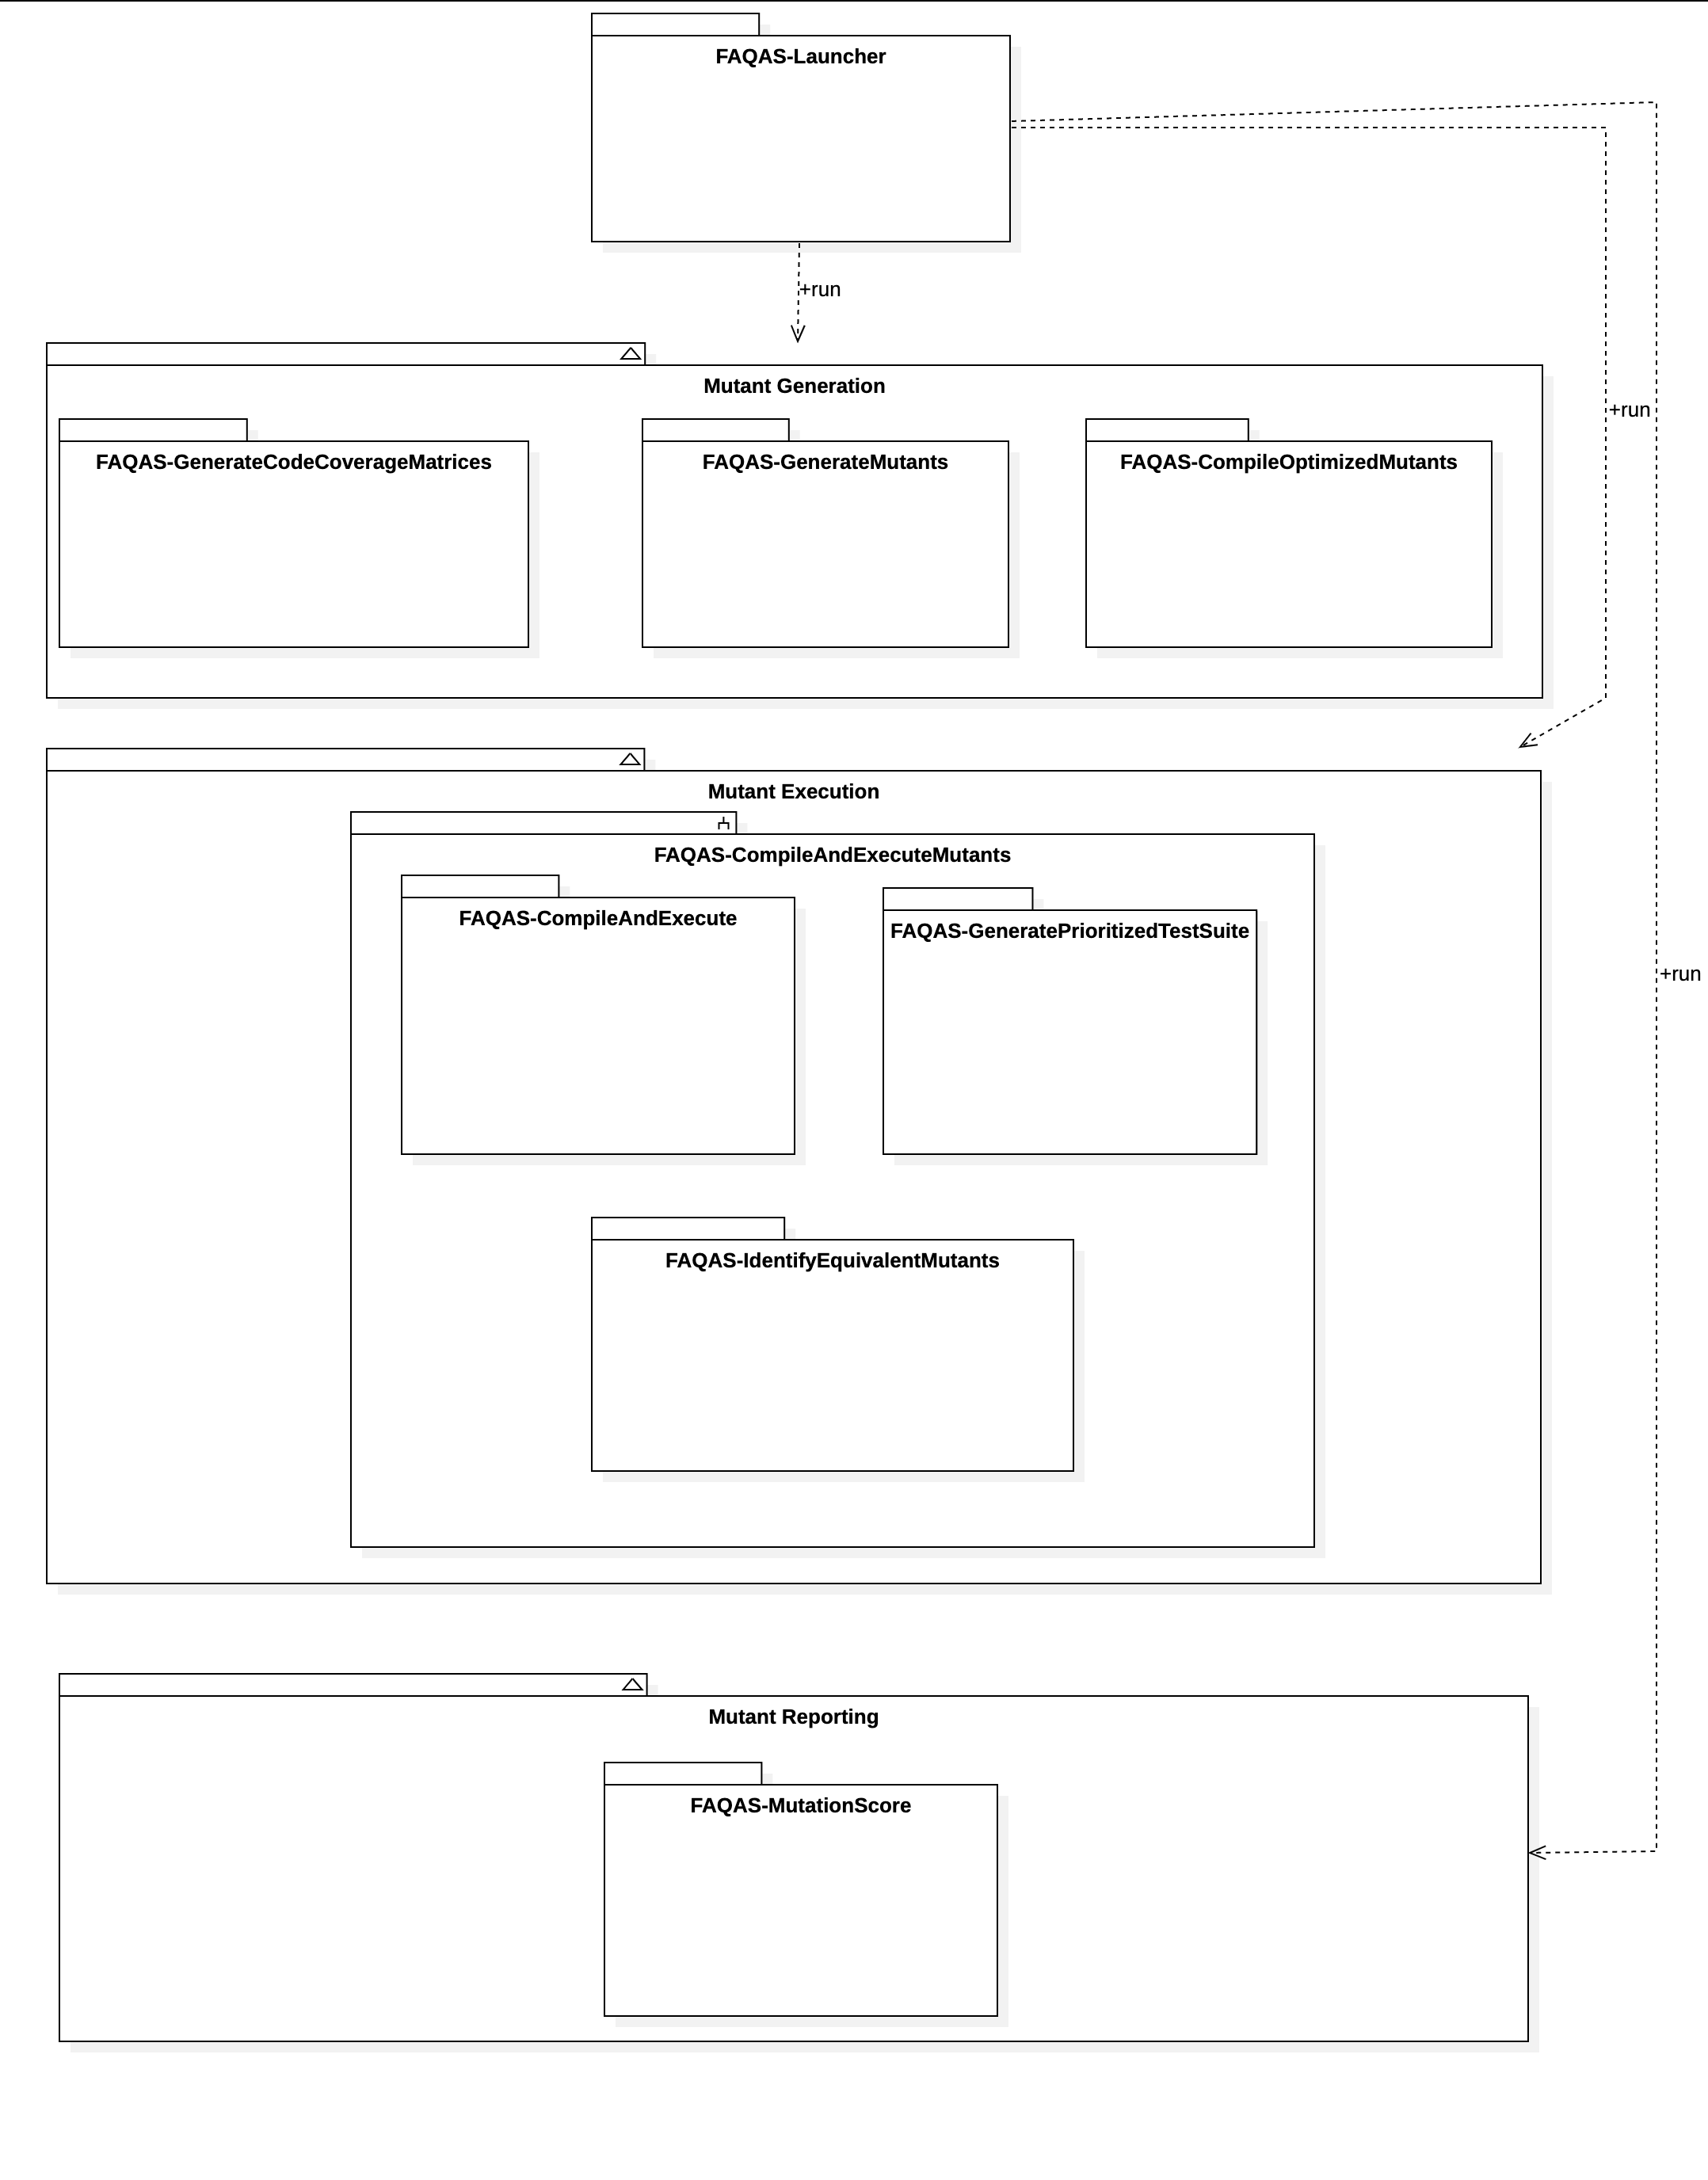
\includegraphics[width=0.8\textwidth]{images/static_architecture.png}
      \caption{UML Architecture diagram of MASS.}
      \label{fig:architecture_diagram}
\end{figure}

The architecture of the code-driven mutation analysis toolset (i.e., MASS)  is drafted in Figure~\ref{fig:architecture_diagram}.
Figure~\ref{fig:architecture_diagram} relies on UML package diagram notation.

As depicted in Figure~\ref{fig:architecture_diagram}, the architecture of the component is divided in three packages, which are named \textit{Mutant Generation}, \textit{Mutant Execution}, and \textit{Mutant Reporting}. Also, it includes the entry point \textit{FAQAS-Launcher}.

The package \textit{Mutant Generation} implements the features concerning (1) the collection of code coverage, (2) the generation of mutants, and (3) the discarding of equivalent and redundant mutants based on compiler optimisations.

The package \textit{Mutant Execution} implements the features regarding the compilation and execution of mutants. Note that this layer implements also the strategies for mutation sampling and reduction of the test suites.

The package \textit{Mutant Reporting} implements the features for the generation of the mutation analysis reports including the mutation score.



\clearpage

\subsection{Software components design}

\begin{figure}[tb]
  \centering
	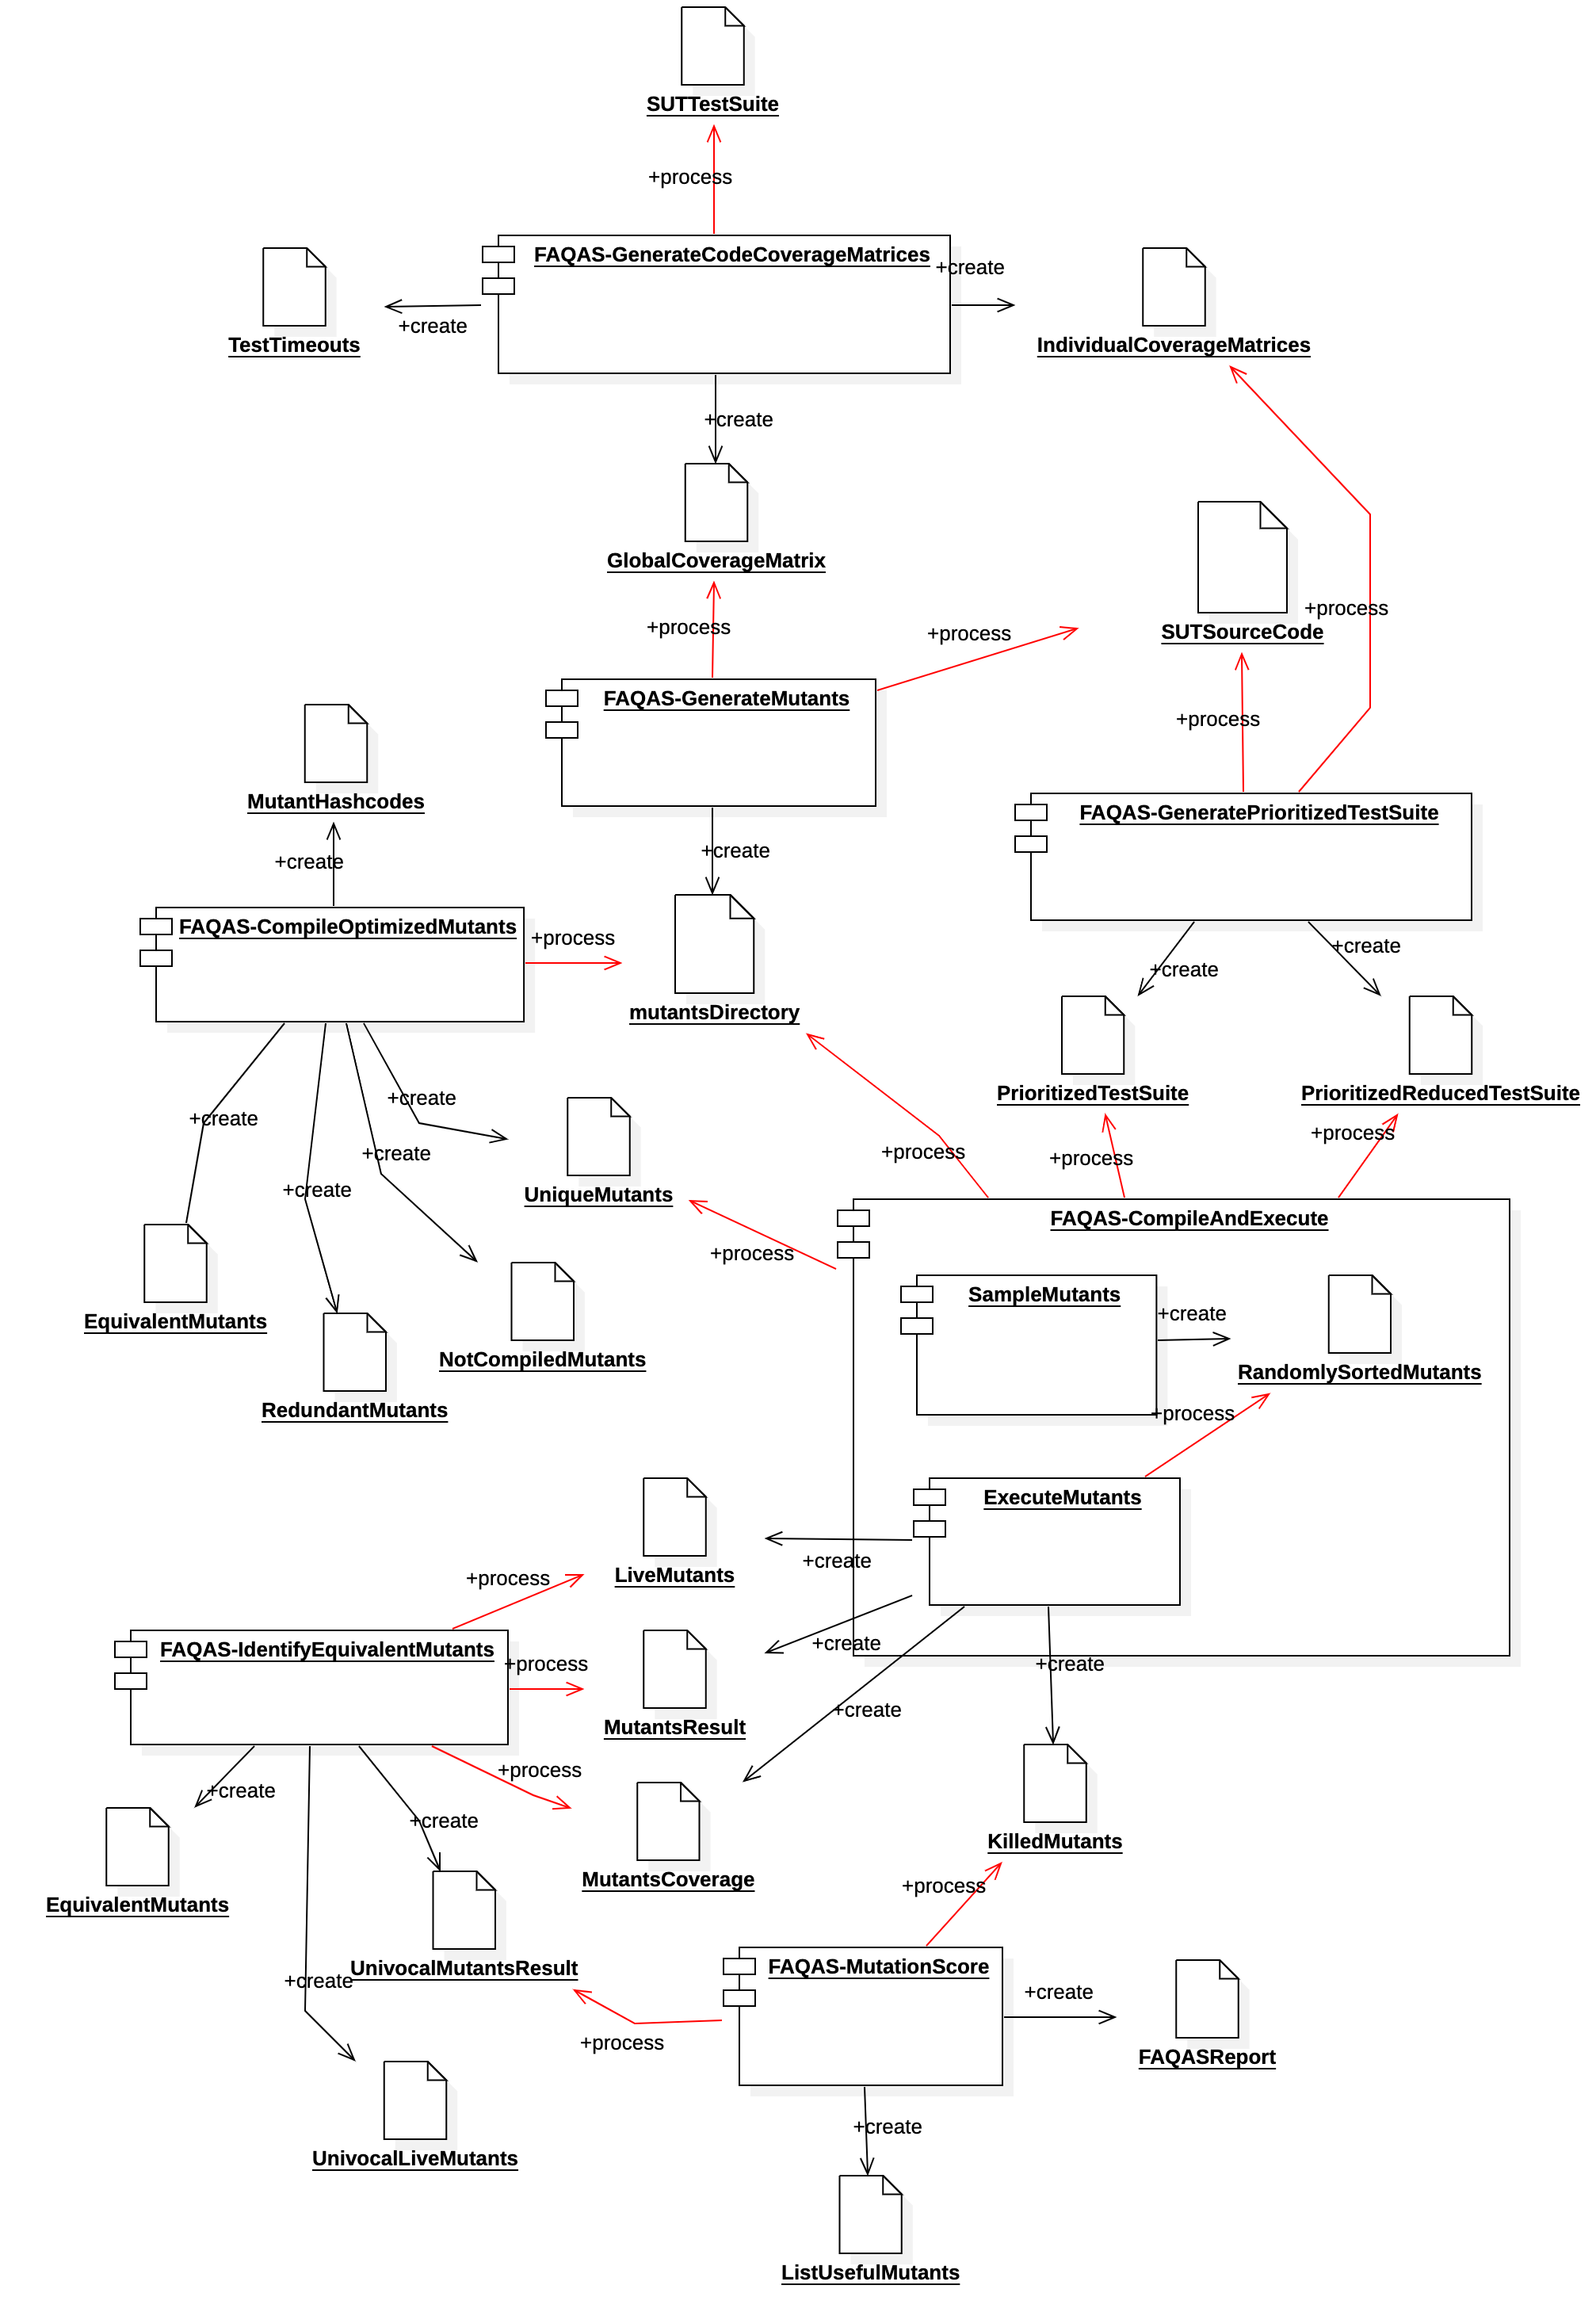
\includegraphics[width=0.9\textwidth]{images/component.png}
      \caption{UML Component diagram of the code-driven mutation testing component to evaluate test suite effectiveness.}
      \label{fig:component_diagram}
%      \DONE{Replace "creates" with "create".}
%            \DONE{Maybe yo can make "process" arrows red to make the data-flow more explicit?}
\end{figure}

The components of MASS are drafted in Figure~\ref{fig:component_diagram}. Figure~\ref{fig:component_diagram} relies on UML component diagram notation.

As shown in Figure~\ref{fig:component_diagram}, the software is composed by the following components:

\begin{itemize}
	\item \textit{FAQAS-GenerateCodeCoverageMatrices}: this component processes the SUT test suite and generates the files \textit{GlobalCoverageMatrix}, \textit{IndividualCoverageMatrices}, and \textit{TestTimeouts}. The information produced by the component is mainly processed by the \textit{FAQAS-GenerateMutants} component.

	\item \textit{FAQAS-GenerateMutants}: This component processes the SUT source code and the \textit{GlobalCoverageMatrix} file, and generates the mutants directory.

	\item \textit{FAQAS-GeneratePrioritizedTestSuite}: this component processes the source code and the \textit{IndividualCoverageMatrices}, and produces two files: the \textit{PrioritizedTestSuite} and the \textit{PrioritizedReducedTestSuite}.

	\item \textit{FAQAS-CompileOptimizedMutants}: this component processes the mutants directory and produces five files:
	\begin{itemize}
		\item \textit{MutantHashcodes}: file containing the list of hash-codes for each mutant
		\item \textit{UniqueMutants}: file containing the list of nonequivalent and nonredundant mutants
		\item \textit{EquivalentMutants}: file containing the list of equivalent mutants
		\item \textit{RedundantMutants}: file containing the list of redundant mutants
		\item \textit{NotCompiledMutants}: file containing the list of non-compiled mutants
	\end{itemize}
	\item \textit{FAQAS-CompileAndExecute}: this component is composed by two sub-components:
		\begin{itemize}
			\item \textit{SampleMutants}: this component processes the file \textit{UniqueMutants} and generates the file \textit{RandomlySortedMutants}
			\item \textit{ExecuteMutants}: this component processes the file \textit{RandomlySortedMutants}, and execute the mutants (according to the strategy selected by the end-user). It produces the following files:
			\begin{itemize}
				\item \textit{LiveMutants}: file containing the list of live mutants
				\item \textit{KilledMutants}: file containing the list of killed mutants
				\item \textit{MutantsResults}: file containing the mutation traces
				\item \textit{MutantsCoverage}: folder containing the coverage for every mutant
			\end{itemize}
		\end{itemize}
	\item \textit{FAQAS-IdentifyEquivalentMutants}: this component processes the files \textit{LiveMutants}, \textit{MutantsResults}, and \textit{MutantsCoverage}, and generates the files \textit{EquivalentMutants}, \textit{UnivocalLiveMutants}, and \textit{UnivocalMutantsResults}, that is, it filters equivalent mutants from the mutation execution process.

	\item \textit{FAQAS-MutationScore}: this component processes the \textit{UnivocalMutantsResults} and the \textit{KilledMutants} files and produces the files \textit{FAQASReport} and \textit{LiveUsefulMutants}.
\end{itemize}

\clearpage

%\section{Software dynamic architecture}

\subsection{Software Behavior}

%Concerning the dynamic behavior of the software, we introduce in the following descriptions for each of the four components of the \FAQAS: the Code-Driven Test Suite Evaluation and Augmentation, and the Data-Driven Test Suite Evaluation and Augmentation.

%\subsection{Code-Driven Test Suite Evaluation}

\begin{figure}[h]
  \centering
	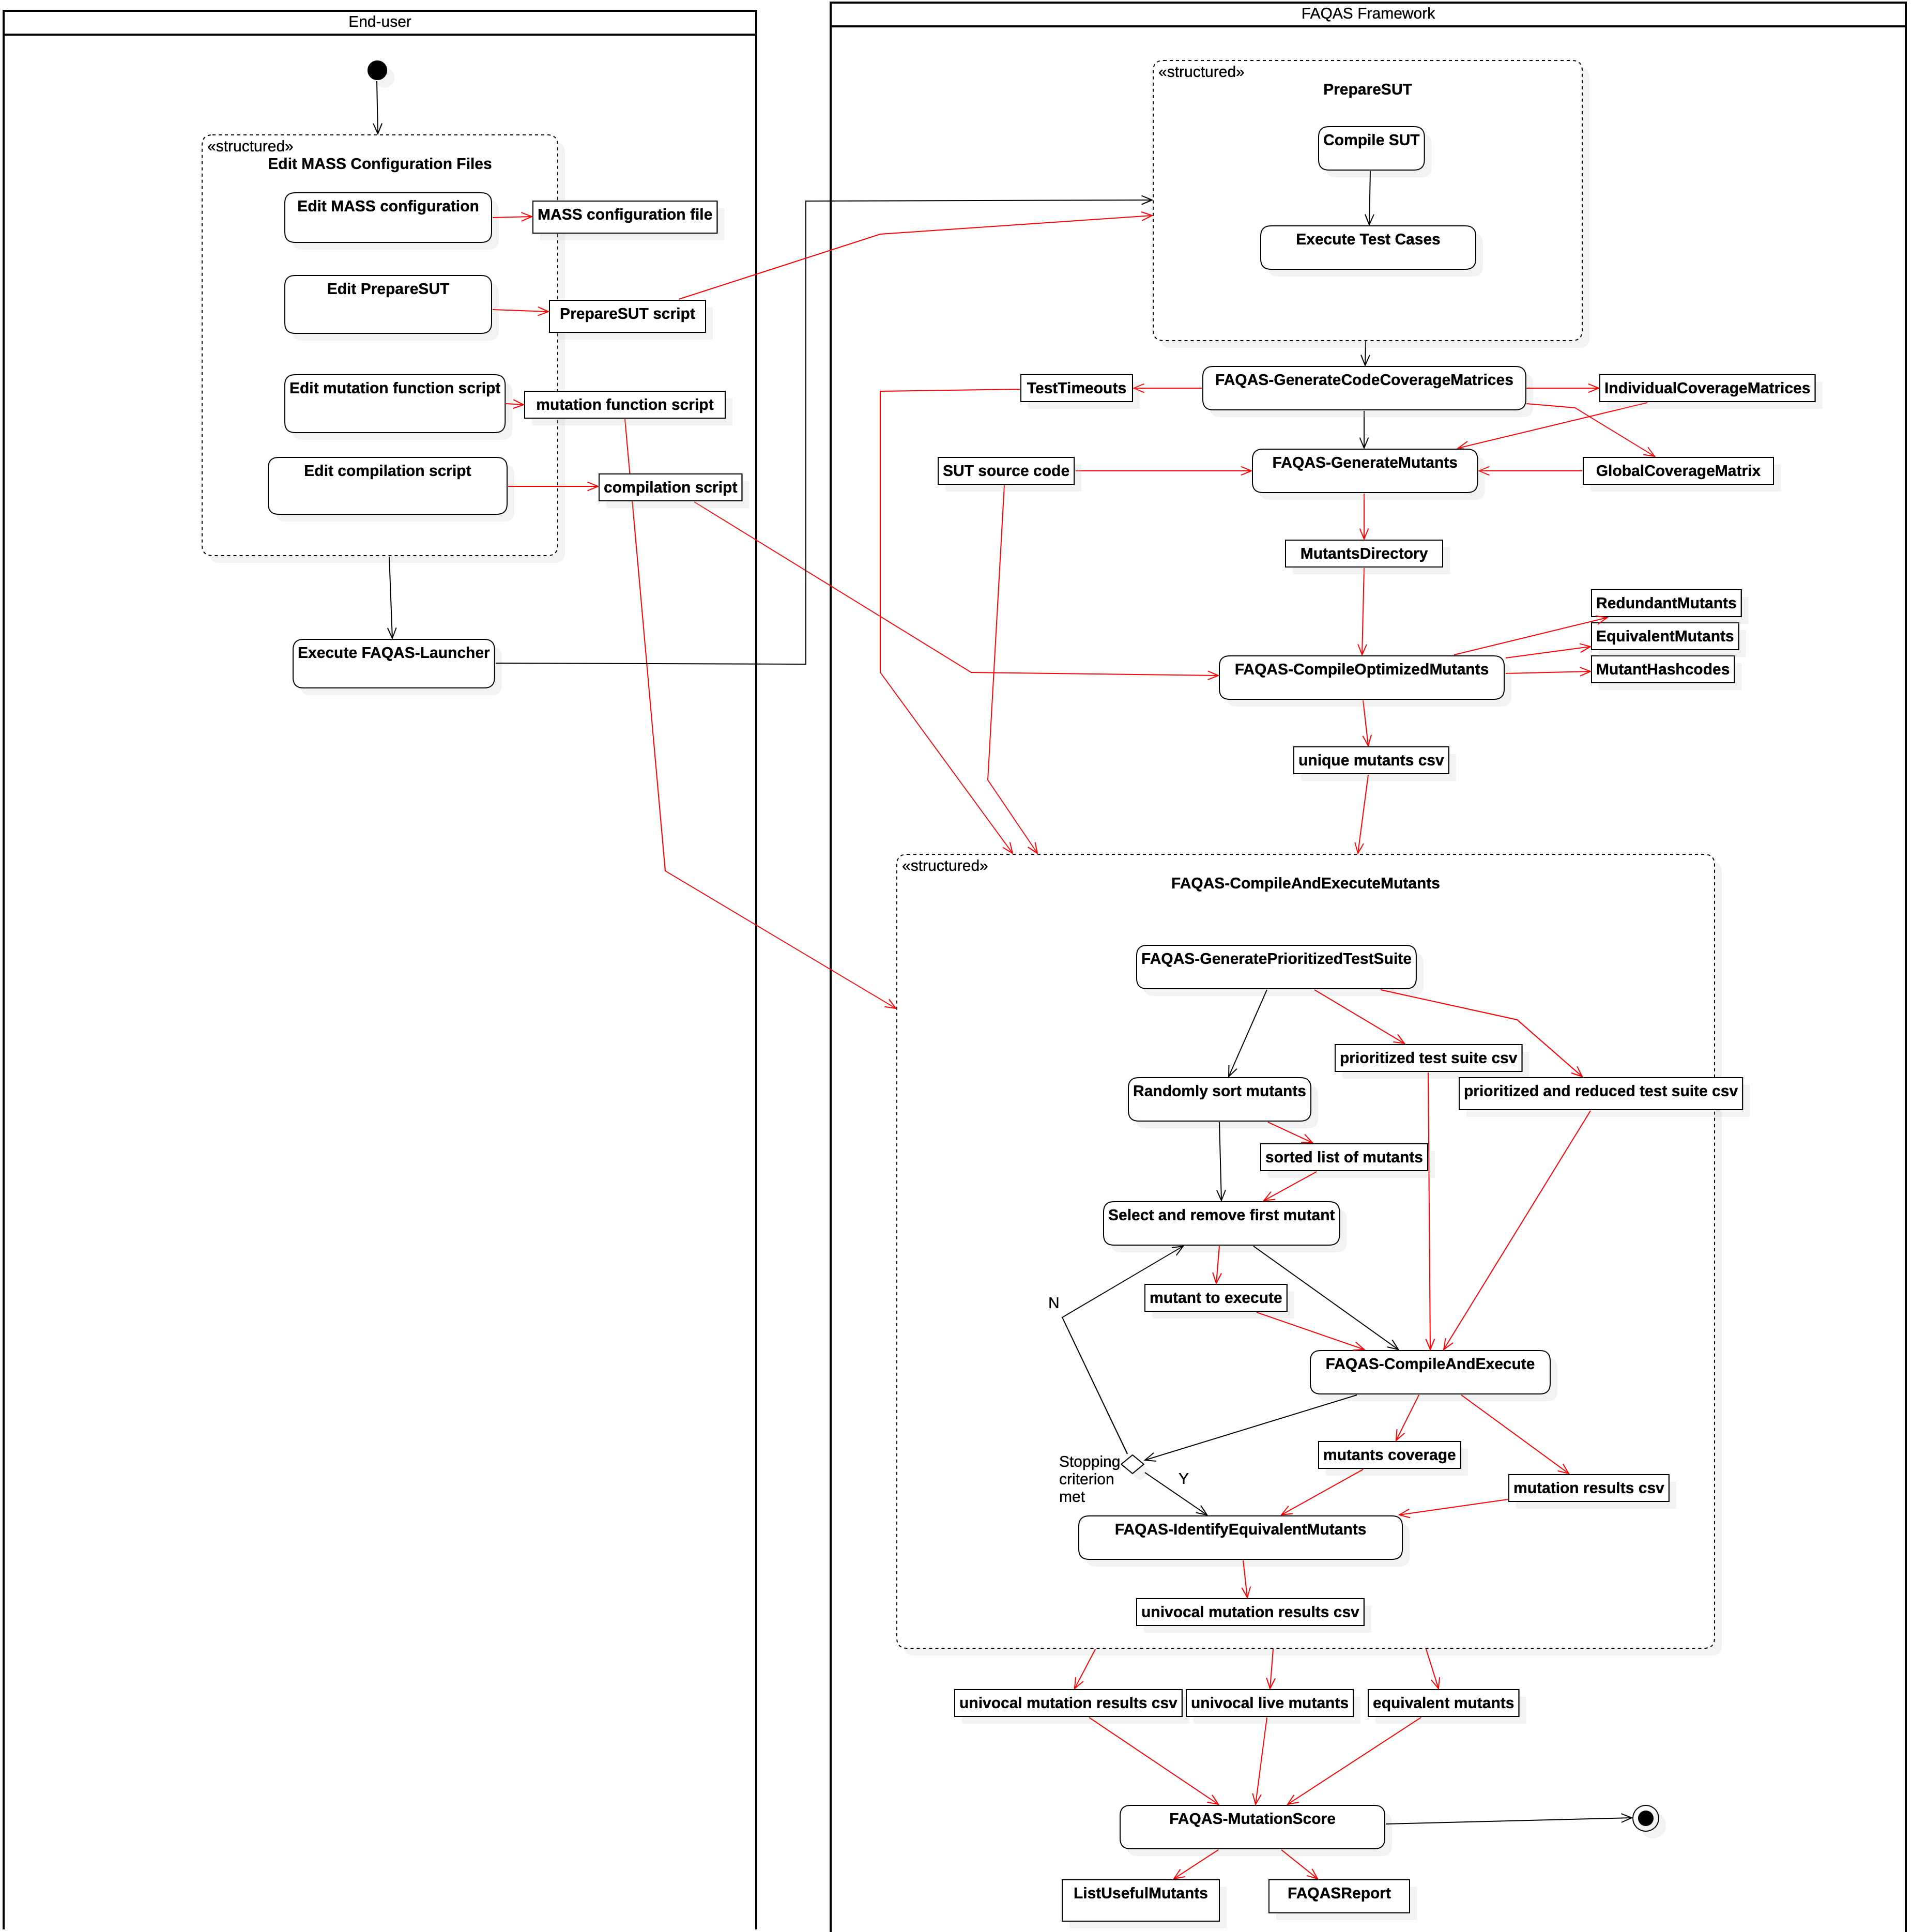
\includegraphics[width=\textwidth]{images/CodeDrivenTestSuiteEvaluation.png}
      \caption{Overview of the code-driven mutation testing process to evaluate test suite effectiveness.}
      \label{fig:process:codeDriven:evaluation}
\end{figure}


MASS implements the process for the evaluation of test suite effectiveness, drafted in Figure~\ref{fig:process:codeDriven:evaluation}. Figure~\ref{fig:process:codeDriven:evaluation} relies on UML activity diagram notation. In Figure~\ref{fig:process:codeDriven:evaluation} the execution of specific software artefacts from the end user is made explicit. Also, we use black arrows to draw control-flow, red arrows for data-flow. In the following, we further describe the evaluation of test suite effectiveness process.


The activity \emph{Edit MASS Configuration Files} indicates that the engineers must configure and perform the following activities:
\begin{itemize}
	\item Edit MASS configuration file: general configuration file
	\item Edit PrepareSUT script: script that compiles the SUT and executes the SUT test suite. In particular,  it extends the \emph{test suite script} for the SUT to store the code coverage of each single test case separately. This is achieved by adding a call to a dedicated bash script provided by FAQAS (\emph{FAQAS-CollectCodeCoverage}) after the execution of every test case.
	\item Edit Mutation function script: implementation of the function that executes the SUT test cases and decides whether a test case has been killed.
	\item Edit compilation script: modified version of the original build script to be used by \emph{FAQAS-}\emph{Compile\-OptimizedMutants}. The compilation script must be modified by:
	\begin{itemize}
	\item Removing debugging flags
	\item Removing coverage flags
	\item Adding a placeholder for the compiler optimization option
	\item Adding a 'sort' command in the source dependency list to ensure that source files are always compiled in the same order
	\end{itemize}
\end{itemize}

%\DONE{I think \emph{Prepare compilation scripts} is now covered by \emph{Edit compilation script} in the End-user part. I suggest to remove it from \emph{FAQAS-Framework part}. Also add the information above to the description of \emph{Edit compilation script}.}

The activity \emph{Compile SUT} in Figure~\ref{fig:process:codeDriven:evaluation} indicates that \MASS shall compile the SUT with coverage options enabled.

% The activity \emph{Prepare test scripts} in Figure~\ref{fig:process:codeDriven:evaluation} concerns extending the \emph{test suite script} for the SUT to store the code coverage of each single test case separately. This is achieved by adding a call to a dedicated bash script provided by FAQAS (\emph{FAQAS-CollectCodeCoverage}) after the execution of every test case.

%\DONE{The \emph{Prepare test scripts} is manual. Thus it should not be part of FAQAS-Framework. However, I think it has been replaced by "Edit compilation script" or "Edit PrepareSUT", no?}

The activity \emph{Execute test cases} in Figure~\ref{fig:process:codeDriven:evaluation} concerns the execution of the test cases following the practice for the SUT (e.g., running the command \texttt{make test}).

The activity \emph{Execute FAQAS-GenerateCodeCoverageMatrix} in Figure~\ref{fig:process:codeDriven:evaluation} concerns the execution of a program delivered with the FAQAS framework (i.e., FAQAS-GenerateCodeCoverageMatrix).

%\DONE{Some output arrows departing from FAQAS-GenerateCodeCoverageMatrix are missing}

The activity \emph{Execute FAQAS-GenerateCodeCoverageMatrix} in Figure~\ref{fig:process:codeDriven:evaluation} generates a set of files:
\begin{itemize}
\item one csv file referred to as \emph{global coverage matrix}, which indicates, for every line of code of the SUT, the ID of the test cases that cover the line of code;
\item a number of files  referred to as \emph{individual coverage matrices}, one for each test case of the SUT. Each file indicates, for every line of code of the SUT, the number of times it has been covered during a single execution of the test case;
\item one file (\emph{TestTimeouts}) specifying, for each test case, a timeout value after which we shall consider a test case as hanging. The timeout value is generated by the system by triplicating the time taken by a test case launched in activity \emph{Execute test cases}.
\end{itemize}

Activity \emph{Execute FAQAS-GenerateMutants} in Figure~\ref{fig:process:codeDriven:evaluation} concerns the execution of the program \emph{FAQAS-GenerateMutants}.

The program \emph{FAQAS-GenerateMutants} automatically generates a number of copies of each source file. Each copy contains one mutant.

\emph{FAQAS-GenerateMutants} mutates source files implemented with C/C++ programming languages.

%\DONE{What about C++? I think we promised it...}
%\OSCAR{We haven't tried yet... since all case studies are written in C.}

\emph{FAQAS-GenerateMutants} generates mutants by applying a set of mutation operators that can be selected by the end-users.

\emph{FAQAS-GenerateMutants} implements the set of operators listed in Table~\ref{table:operators}

% !TEX root =  ../Main.tex

\newcommand{\op}{\mathit{op}}
\newcommand{\ArithmeticSet}{ \texttt{+}, \texttt{-}, \texttt{*}, \texttt{/}, \texttt{\%} }
\newcommand{\LogicalSet}{ \texttt{&&}, \texttt{||} }
\newcommand{\RelationalSet}{ \texttt{>}, \texttt{>=}, \texttt{<}, \texttt{<=}, \texttt{==}, \texttt{!=} }
\newcommand{\BitWiseSet}{ \texttt{\&}, \texttt{|}, \land }
\newcommand{\ShiftSet}{ \texttt{>>}, \texttt{<<} }


\begin{table}[h]
\caption{Implemented set of mutation operators.}
\label{table:operators} 
\centering
\scriptsize
\begin{tabular}{|@{}p{4mm}@{}|@{}p{2cm}@{\hspace{1pt}}|@{}p{11.1cm}@{}|}
\hline
&\textbf{Operator} & \textbf{Description$^{*}$} \\
\hline
\multirow{7}{*}{\rotatebox{90}{\emph{Sufficient Set}}}&ABS               & $\{(v, -v)\}$	\\
\cline{2-3}
&AOR               & $\{(\op_1, op_2) \,|\, \op_1, \op_2 \in \{ \ArithmeticSet \} \land \op_1 \neq \op_2 \} $       \\
&    			  & $\{(\op_1, \op_2) \,|\, \op_1, \op_2 \in \{\texttt{+=}, \texttt{-=}, \texttt{*=}, \texttt{/=}, \texttt{\%} \texttt{=}\} \land \op_1 \neq \op_2 \} $       \\
\cline{2-3}
&ICR               & $\{i, x) \,|\, x \in \{1, -1, 0, i + 1, i - 1, -i\}\}$           \\
\cline{2-3}
&LCR               & $\{(\op_1, \op_2) \,|\, \op_1, \op_2 \in \{ \texttt{\&\&}, || \} \land \op_1 \neq \op_2 \}$            \\
&				  & $\{(\op_1, \op_2) \,|\, \op_1, \op_2 \in \{ \texttt{\&=}, \texttt{|=}, \texttt{\&=}\} \land \op_1 \neq \op_2 \}$            \\
&				  & $\{(\op_1, \op_2) \,|\, \op_1, \op_2 \in \{ \texttt{\&}, \texttt{|}, \texttt{\&\&}\} \land \op_1 \neq \op_2 \}$            \\
\cline{2-3}
&ROR               & $\{(\op_1, \op_2) \,|\, \op_1, \op_2 \in \{ \RelationalSet \}\}$            \\
&				  & $\{ (e, !(e)) \,|\, e \in \{\texttt{if(e)}, \texttt{while(e)}\} \}$ \\
\cline{2-3}
&SDL               & $\{(s, \texttt{remove}(s))\}$            \\
\cline{2-3}
&UOI               & $\{ (v, \texttt{--}v), (v, v\texttt{--}), (v, \texttt{++}v), (v, v\texttt{++}) \}$            \\   
\hline
\hline
\multirow{5}{*}{\rotatebox{90}{\emph{OODL}}}&AOD               & $\{((t_1\,op\,t_2), t_1), ((t_1\,op\,t_2), t_2) \,|\, op \in \{ \ArithmeticSet \} $       \\ 
\cline{2-3}
&LOD               & $\{((t_1\,op\,t_2), t_1), ((t_1\,op\,t_2), t_2) \,|\, op \in \{  \} \}$       \\ 
\cline{2-3}
&ROD               & $\{((t_1\,op\,t_2), t_1), ((t_1\,op\,t_2), t_2) \,|\, op \in \{ \RelationalSet \} \}$       \\ 
\cline{2-3}
&BOD               & $\{((t_1\,op\,t_2), t_1), ((t_1\,op\,t_2), t_2) \,|\, op \in \{ \BitWiseSet \} \}$       \\ 
\cline{2-3}
&SOD               & $\{((t_1\,op\,t_2), t_1), ((t_1\,op\,t_2), t_2) \,|\, op \in \{ \ShiftSet \} \}$       \\ 
%\hline
%COR               & $\{(\op_1, \op_2) \,|\, \op_1, \op_2 \in \{ \texttt{\&\&}, \texttt{||}, \land \} \land \op_1 \neq \op_2 \}$            \\
\hline
\hline
\multirow{3}{*}{\rotatebox{90}{\emph{Other}}}&LVR			& $\{(l_1, l_2) \,|\, (l_1, l_2) \in \{(0,-1), (l_1,-l_1), (l_1, 0), (\mathit{true}, \mathit{false}), (\mathit{false}, \mathit{true})\}\}$\\
&&\\
&&\\
\hline
\end{tabular}

$^{*}$Each pair in parenthesis shows how a program element is modified by the mutation operator. Th eleft element of the pair is replaced with the right element. We follow standard syntax~\cite{kintis2018effective}. Program elements are literals ($l$), integer literals ($i$), boolean expressions ($e$), operators ($\op$), statements ($s$), variables ($v$), and terms ( $t_i$, which might be either variables or literals).
\end{table}

\emph{FAQAS-GenerateMutants} generates as output a directory tree (\emph{MutantsDirectory} in Figure~\ref{fig:process:codeDriven:evaluation}) that follows the structure of the source directory tree of the SUT. However, every source file is replaced by a folder; the folder has the same name of the file. The folder contains all the mutants generated for that file. Every mutant has a name that univocally identifies it. The mutant name results from the conjunction of the following information:
source file name, mutated function name, mutated line, mutation operator name, mutation operation, mutated ``column'' (i.e., char position from the beginning of the line).
In the following, we report the structure of the output directory generated for a program

\begin{verbatim}
./src/store/vmem/vmem_checksum_first.c
./src/log/telemetry_appender.c

./src-mutants/store/vmem/vmem_checksum_first/
vmem_checksum_first.mut.145.7_1_13.ROR.vmem_param_load.c
./src-mutants/log/telemetry_appender/
telemetry_appender.mut.116.3_1_18.ROR.gs_log_appender_telem_append_isr.c
\end{verbatim}

%\DONE{The "compilation script" should be an output of \emph{Edit compilation script}}

Activity \emph{Execute FAQAS-CompileOptimizedMutants} in Figure~\ref{fig:process:codeDriven:evaluation} concerns the execution of the program \emph{FAQAS-CompileOptimizedMutants}.

The program \emph{FAQAS-CompileOptimizedMutants} compiles every mutant multiple times, once for every compiler optimization option selected by the end-user. It implements the pseudocode in Figure~\ref{alg:CompileOptimizedMutants}.

\begin{figure}[h]
\begin{algorithmic}[1]

%\footnotesize
\scriptsize

\Require \emph{OPT}, the set of compiler optimization options specified by the end-user
\Require \emph{MutantsDir}, path of the directory tree containing the mutants
\Require \emph{SUTsources}, path of the folder containing the sources of the SUT
\Require \emph{CompilatonCommand}, the command to execute to compile the original software

\Ensure \emph{hashcodes csv}, a csv file containing for every mutant, for every option, the SHA512 hashcode of the generated executable

\Ensure \emph{unique mutants}, a csv file containing the list of unique mutants. Unique mutants are mutants that are not equivalent and not redundant. See D2 for details.

\For {OPT in OPTS}
\For {Mutant in MutantsDir}
\State Compile \emph{Mutant} with program \emph{FAQAS-CompileAndExecute}
\State Generate a SHA512 hash of the generated executable
\State Put the generated SHA512 hash in the \emph{hashcodes csv} file
\EndFor
\EndFor

\State Process \emph{hashcodes csv} and identify the \emph{unique mutants}
\State Save the list of \emph{unique mutants} in the output file \emph{unique mutants csv}

\end{algorithmic}
\caption{FAQAS-CompileOptimizedMutants: Algorithm for compiling mutants with multiple optimization options}
\label{alg:CompileOptimizedMutants}
\end{figure}


Activity \emph{Execute FAQAS-Compile\-And\-Execute\-Mutants} in Figure~\ref{fig:process:codeDriven:evaluation} concerns the execution of the program \emph{FAQAS-Compile\-And\-Execute\-Mutants}.

The program \emph{FAQAS-CompileAndExecuteMutants} iterates over three activities: \emph{FAQAS-Generate\-Prioritized\-Test\-Suite}, \emph{FAQAS-CompileAndExecute}, \emph{FAQAS-IdentifyEquivalentMutants}. Each activity is implemented by a dedicated executable program that is invoked automatically by \emph{FAQAS-CompileAndExecuteMutants} without user intervention.

The program \emph{FAQAS-CompileAndExecuteMutants} takes as inputs the \emph{mutants selection configuration}, the \emph{unique mutants csv}, the path of the \emph{SUT source folder}, the \emph{command to execute test cases}, and the \emph{path to the folder containing the test coverage matrices}.

The program \emph{FAQAS-CompileAndExecuteMutants} implements the four mutants selection strategies described in D2: \emph{all mutants}, \emph{proportional uniform sampling}, \emph{proportional method-based sampling}, \emph{uniform fixed-size sampling}, and \emph{uniform FSCI sampling}.

The \emph{mutants sampling configuration} consists of the mutants selection strategy and a configuration value that specifies the number of mutants to consider. The format of the value that specifies the number of mutants to consider depends on the strategy; the value may indicate the percentage of mutants to sample (for \emph{proportional uniform sampling}, \emph{proportional method-based sampling}), the number of mutants to sample (for \emph{uniform fixed-size sampling}).

The program\emph{FAQAS-GeneratePrioritizedTestSuite} takes as input the test coverage matrices and generates a file that specifies, for every line of the SUT, the prioritized list of test cases to execute (\emph{prioritized test suite csv}). This file indicates the sequence of test cases that shall be executed when testing a mutant affecting a certain line.

The activity \emph{Randomly sort mutants} indicates that  \emph{FAQAS-CompileAndExecuteMutants} generates a randomly sorted list of mutants. The list contains the mutants in \emph{unique mutants csv}.
In the case of \emph{proportional method-based sampling}, the list contains a set of mutants selected by following the stratified sampling strategy.

The activity \emph{Select and remove first mutant} indicates that  \emph{FAQAS-CompileAndExecuteMutants} selects the first mutant in \emph{sorted list of mutants} and removes it from the list.

The program \emph{FAQAS-CompileAndExecute} compiles a mutant by running the build script of the original program; then it executes the SUT test suite. It follows the algorithm in Figure~\ref{alg:compileAndExecute}.


\begin{figure}[h]
\begin{algorithmic}[1]
\scriptsize
\Require \emph{Mutant}, path of the mutant to compile
\Require \emph{SUTsources}, path of the folder containing the sources of the SUT
\Require \emph{CompilatonCommand}, the command to execute to compile the original software
\Require \emph{TestCommand}, the command to execute to execute a single test case
\Require \emph{TestCases}, the prioritized list of test cases for the line of the mutant
\Require \emph{TestTimeout}, the max execution time that can be taken by the test case
\Ensure \emph{Result} KILLED or LIVE, based on test execution result (i.e., all test cases pass or one test case fails)
\State put \emph{Mutant} in place of the file it has been derived (\emph{original file}), keep the original file in a safe place
\State execute  \emph{CompilatonCommand} inside \emph{SUTsources}
\For {TestCase in TestCases}
\State execute the \emph{TestCase} by running \emph{TestCommand} inside \emph{SUTsources}
% succede qualcosa strano quando scrivi "the"
\If {the \emph{TestCase} fails (i.e., \emph{TestCommand} terminates with an error code)}
\State set \emph{Result} as KILLED
\State break the for loop
\EndIf
\If {the \emph{TestTimeout} expires}
\State set \emph{Result} as KILLED
\State break the for loop
\EndIf
\EndFor
\State move code coverage information in a subfolder of \emph{mutants coverage dir}
\State restore the \emph{original file}
\end{algorithmic}
\caption{FAQAS-CompileAndExecute: Algorithm to compile and test mutants}
\label{alg:compileAndExecute}
\end{figure}

The program \emph{FAQAS-CompileAndExecute} collects the mutation results of every mutant in a file, i.e., \emph{mutation results csv}. It contains, for every mutant, the indication of the mutation result (KILLED/LIVE).

The program \emph{FAQAS-CompileAndExecute} compiles and executes mutants until a termination criterion is met. The termination criterion depends on the mutants selection strategy (see D2 for details):
\begin{itemize}
\item \emph{all mutants}: the list \emph{sorted list of mutants} is empty
\item \emph{proportional uniform sampling}: a number of mutants matching the selected percentage has been executed
\item \emph{proportional method-based sampling}: the list \emph{sorted list of mutants} is empty
\item \emph{uniform fixed-size sampling}: a number of mutants matching the selected value has been executed
\item \emph{uniform FSCI sampling}: the confidence interval computed from \emph{mutation results csv} is smaller than the length specified by the user.
\end{itemize}

The program \emph{FAQAS-IdentifyEquivalentMutants} relies on code coverage information stored in \emph{mutants coverage dir} to identify equivalent and redundant mutants using the distance criterion $D_C$ (see D2).

The program \emph{FAQAS-IdentifyEquivalentMutants} generates a copy of \emph{mutation results csv} (i.e., \emph{univocal mutation results csv}) where only mutants that are considered non-equivalent are reported.

The program \emph{FAQAS-MutationScore} concerns the computation of the mutation score based on the mutation results reported in \emph{univocal mutation results csv}, and the production of the two prioritized lists (list A and list B) of live and nonequivalent mutants (see FAQAS-SSS-REQ-051).



\clearpage
\STARTCHANGEDWPT
% !TEX root = MAIN.tex

\section{SEMuS}

\subsection{Software static architecture}

\begin{figure}[tb]
  \centering
  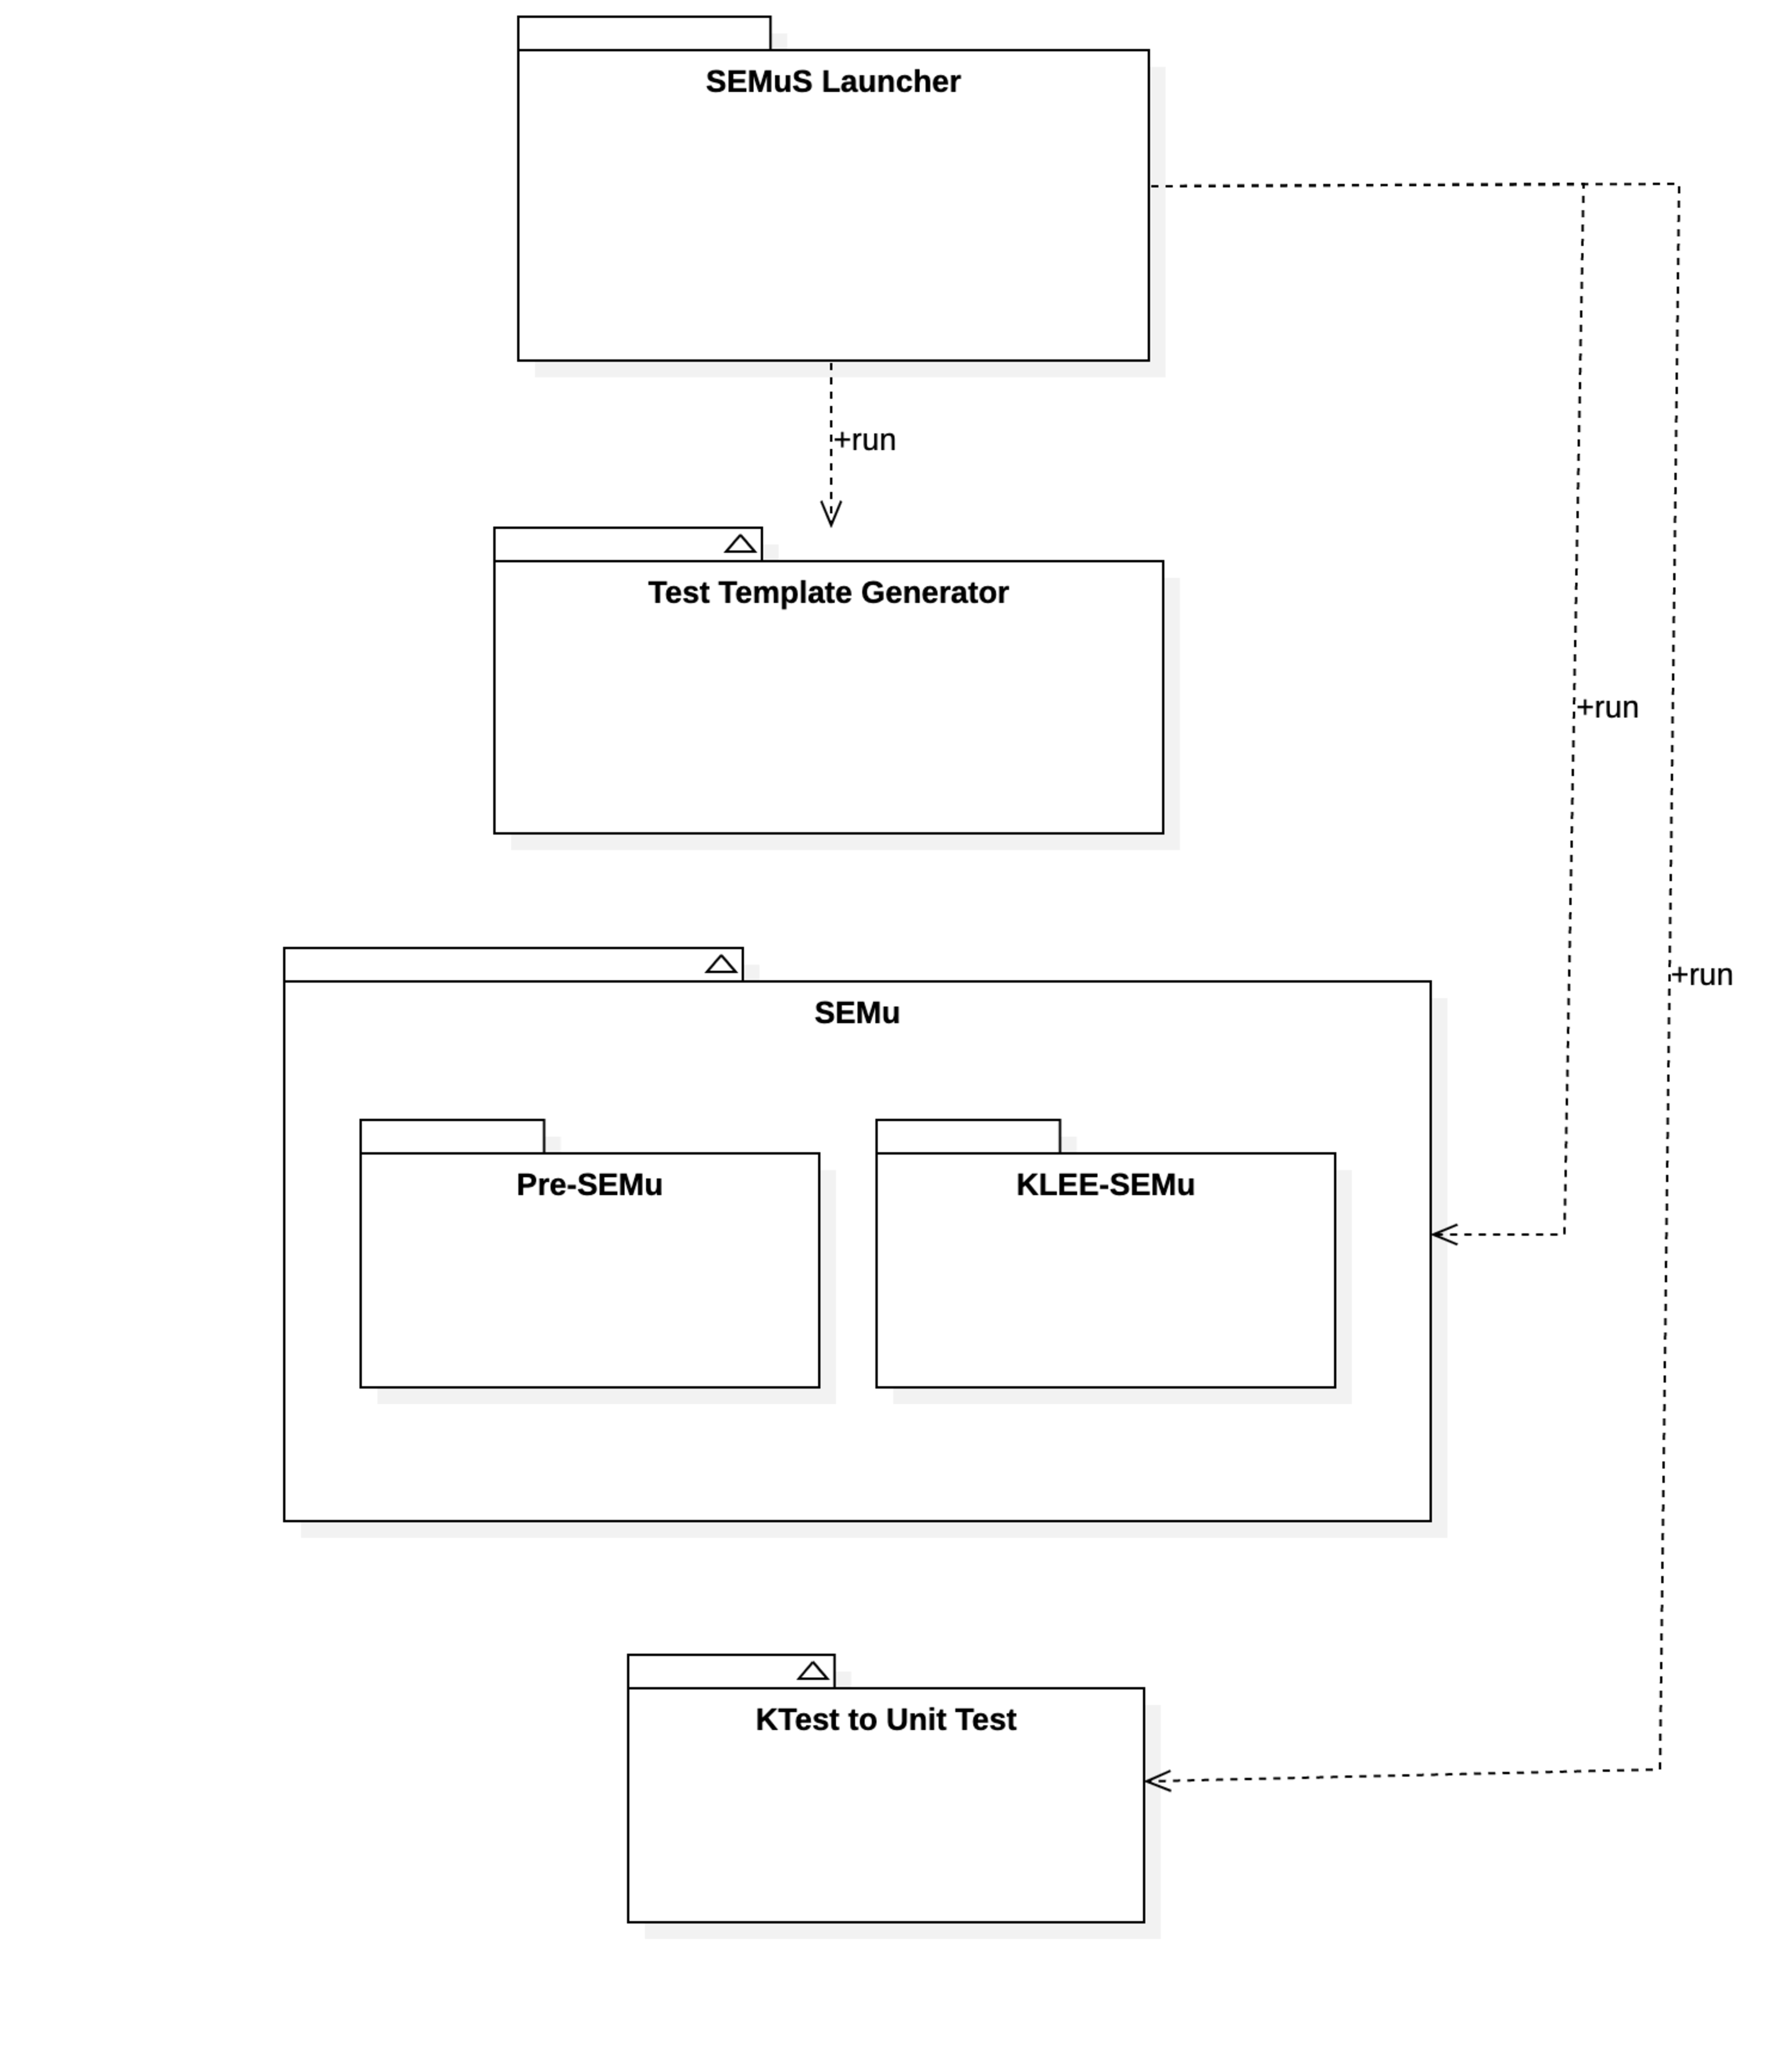
\includegraphics[width=0.6\textwidth]{images/semus-arch-sdd}
      \caption{UML Architecture diagram of SEMuS.}
      \label{fig:architecture_diagram_semus}
\end{figure}

The architecture of the code-driven test suite augmentation toolset (i.e., SEMuS) is drafted in Figure~\ref{fig:architecture_diagram_semus}. The architecture diagram relies on UML package diagram notation.

As specified in Figure~\ref{fig:architecture_diagram_semus}, the architecture of the toolset is divided into three packages:(1) the \emph{Test Template Generator}, (2) the \emph{SEMu}, and (3) the \emph{KTest to Unit Test}. The diagram also includes the entry point of the toolset, which is the \emph{SEMuS Launcher}.

The package \emph{Test Template Generator} implements the features concerning (1) the parsing of the SUT source code, and (2) the generation of test templates for each SUT function.

The package \emph{SEMu} implements the features regarding (1) the generation of the meta mutant, (2) the compilation of the meta mutant, (3) the compilation of the test template, and (4) the invocation of the underlying test generation tool (i.e., KLEE).

The package \emph{KTest to Unit Test} implements the features concerning (1) the parsing of KLEE's output, and (2) the conversion of KLEE tests to C unit test cases.

\subsubsection{Source Code Structure}

SEMuS is delivered as a compressed archive containing a set of source files and an installer. In the following, there is a brief description of the archive's structure once uncompressed:

\begin{itemize}
  \item \texttt{SEMuS/}
    \begin{itemize}
      \item \texttt{underlying\_test\_generation/}: contains the source files of the component that invokes KLEE-SEMu.
      \item \texttt{pre\_semu/}: contains the source files of the component that prepares the meta-mutant file to be processed by KLEE-SEMu.
      \item \texttt{ktest\_to\_unittest/}: contains the source files that implements the component that parses the output of KLEE (i.e., KLEE tests) and converts it to readable C unit test cases.
      \item \texttt{case\_studies/}: contains the configuration files, SUT source codes, and SEMuS launchers for the case studies ASN.1 and MLFS.
      \begin{itemize}
        \item \texttt{scripts/}: contains the configuration files and launchers of the case study.
        \item \texttt{util\_codes/}: folder containing the generated test templates for the case study.
        \item \texttt{WORKSPACE/}: folder containing the SUT source code and list of live mutants.
      \end{itemize}
      \item \texttt{Dockerfile}: text document file that contains all the commands necessary to build a Docker container with all the dependencies of SEMuS.
      \item \texttt{cd\_semu\_docker.sh}: bash script that automates the execution of the toolset through the use of Docker.
      \item \texttt{install\_requirements.sh}: build script that installs SEMuS' requirements.
      \item \texttt{requirements.txt}: list of Python packages to be parsed by \texttt{install\_requirements.sh}.
    \end{itemize}
\end{itemize}

\subsection{Software components design}
\label{sec:component:design:semus}

\begin{figure}[tb]
  \centering
  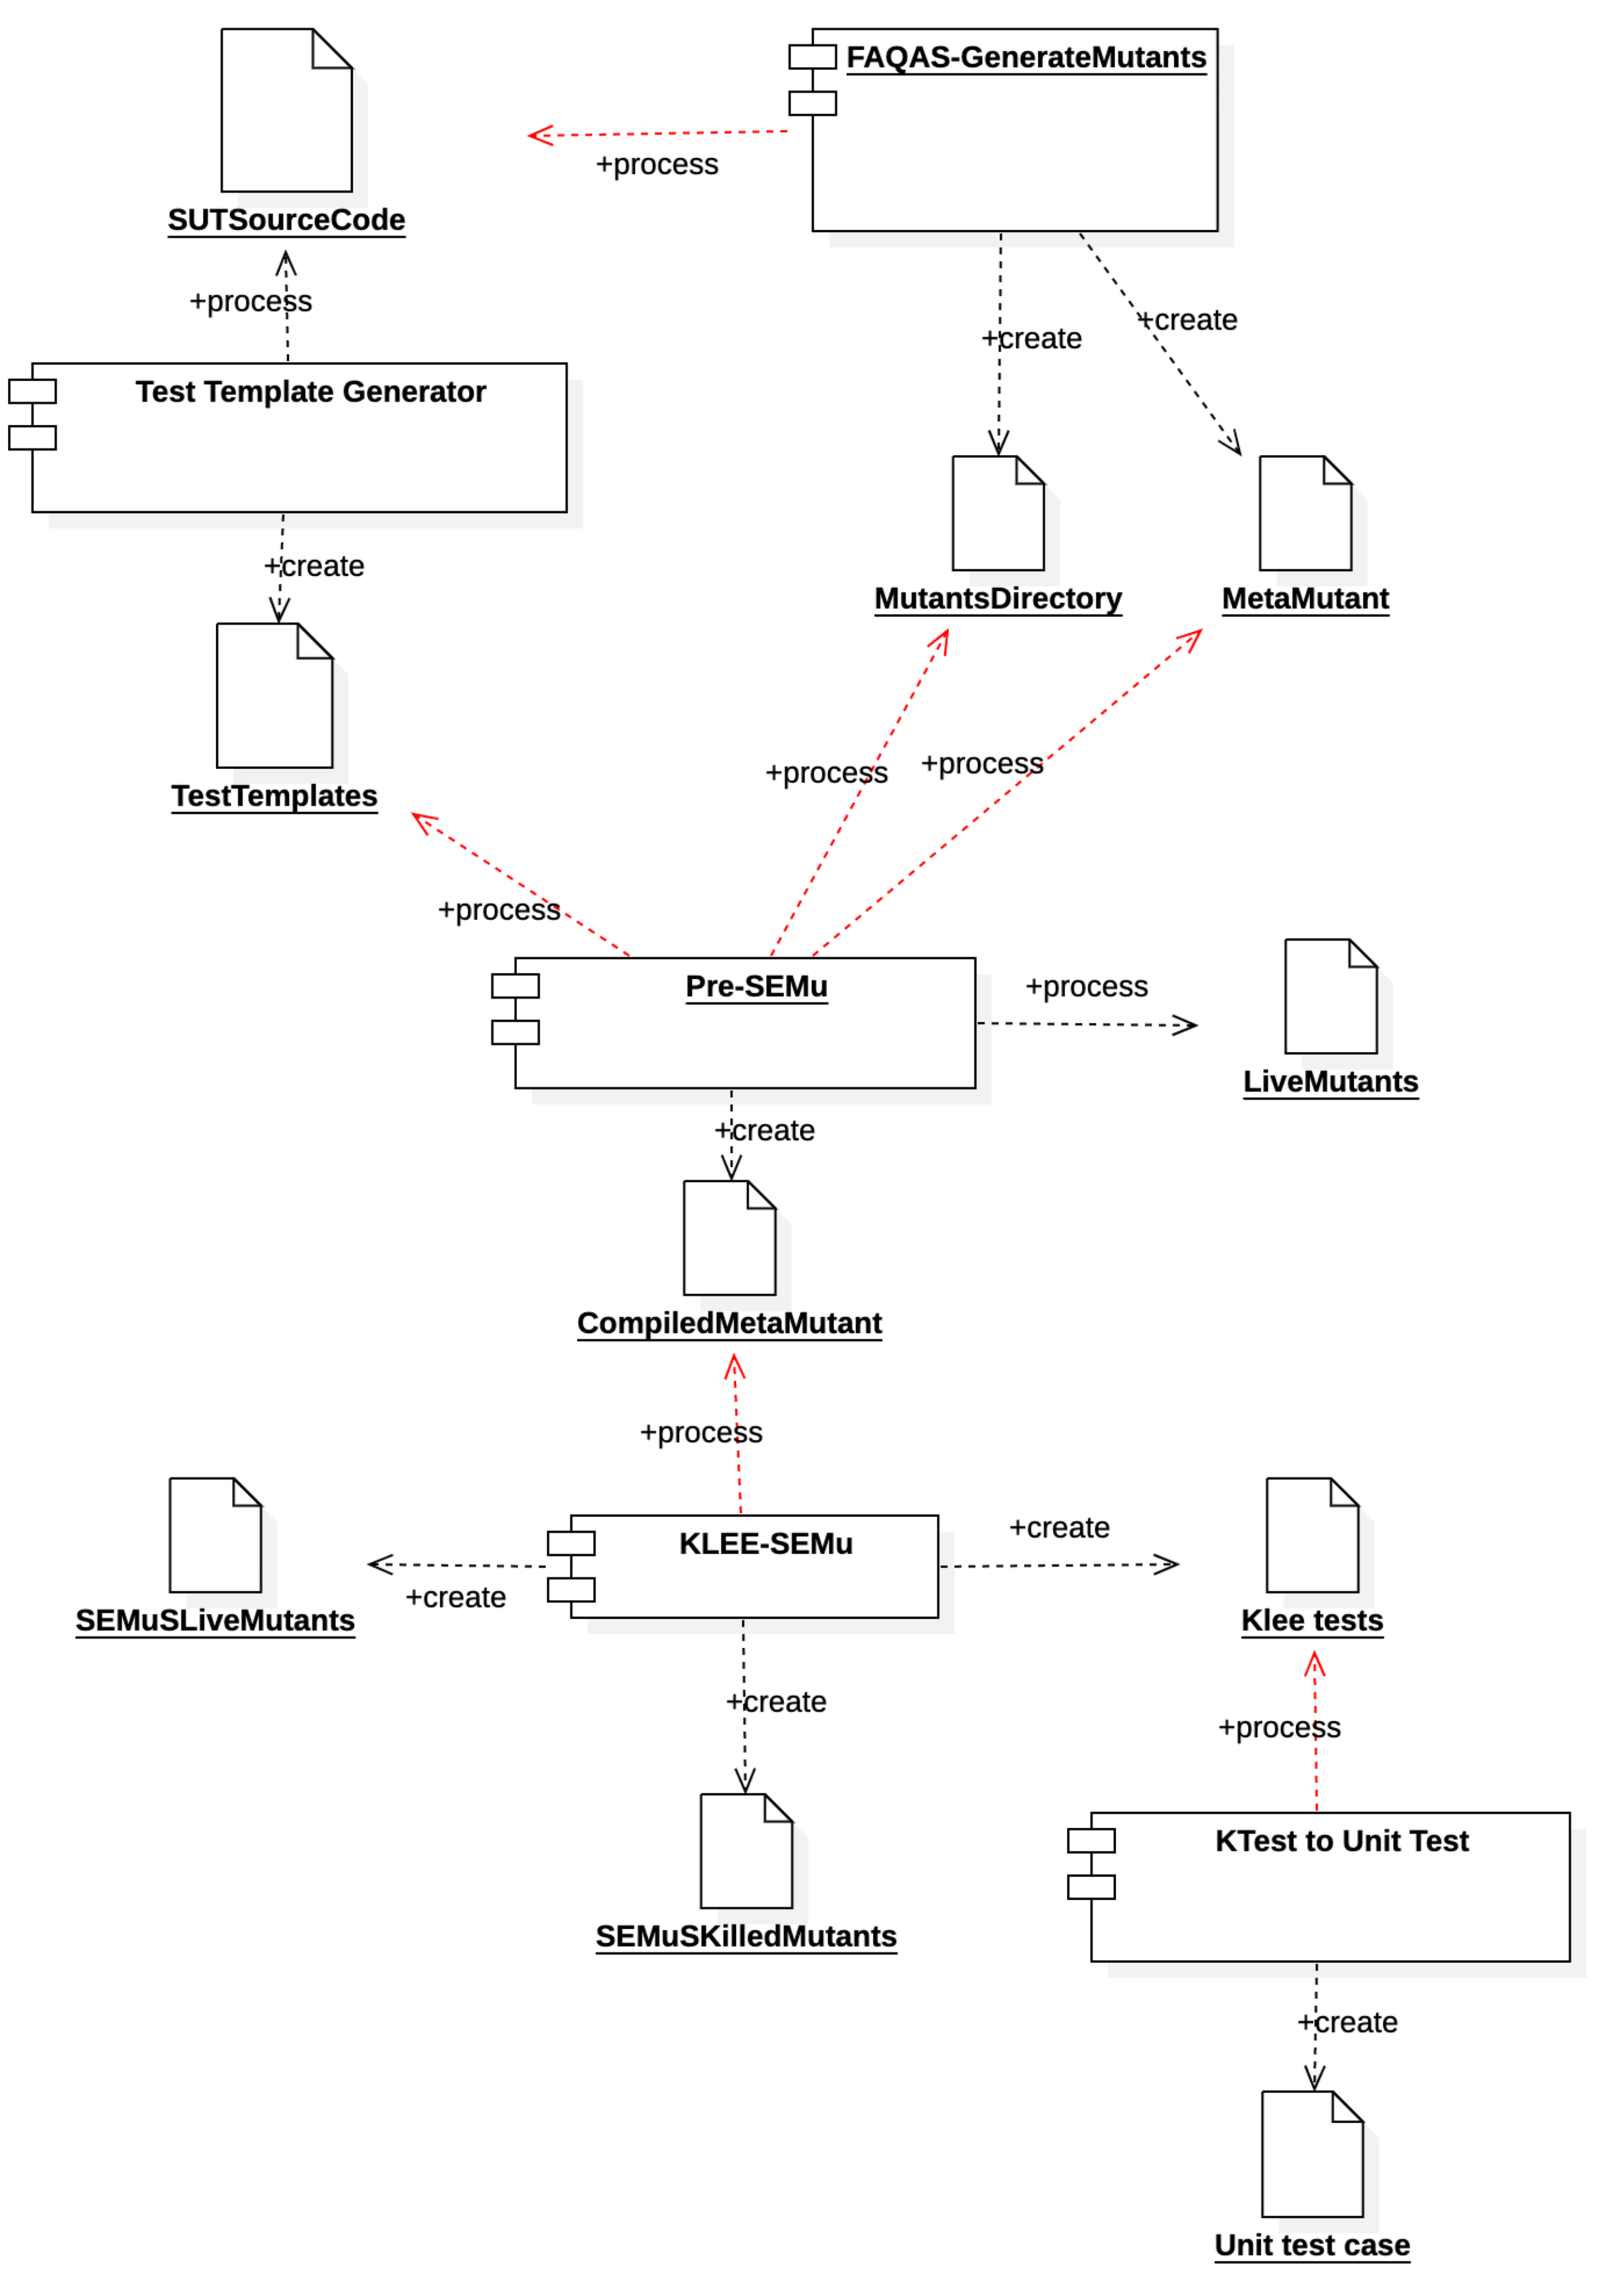
\includegraphics[width=0.7\textwidth]{images/semus-component.pdf}
      \caption{UML Component diagram of the code-driven test suite augmentation toolset (SEMuS). Black arrows show outputs, red arrows show inputs.}
      \label{fig:component_diagram_semus}
\end{figure}


The components of SEMuS are drafted in Figure~\ref{fig:component_diagram_semus}. Figure~\ref{fig:component_diagram_semus} relies on UML component diagram notation.

As shown in Figure~\ref{fig:component_diagram_semus}, the software is composed by the following components:

\begin{itemize}
  \item \emph{Test Template Generator}: this component processes the SUT source code and generates the files \emph{TestTemplates}. The information produces by the component is mainly processed by \emph{Pre-SEMu}.
  \begin{itemize}
    \item \emph{TestTemplates}: test template (i.e., C source file) that contains the wrapping main function for driving the test generation for a specific SUT function.
  \end{itemize}
  \item \emph{FAQAS-GenerateMutants}: this component originally belongs to MASS (see Section~\ref{sec:component:design}), it processes the SUT source code and creates the file \emph{MetaMutant}, and a \emph{MutantsDirectory} including the source code for every mutant targeting a specific source code.
  \begin{itemize}
    \item \emph{MetaMutant}: Source code (i.e., C file) that includes all the mutants for a specific source; every mutated statement is controlled by a switch statement that decides the mutant to be activated during testing.
  \end{itemize}
  \item \emph{Pre-SEMu}: this component processes the files \emph{TestTemplates}, \emph{MetaMutant}, the \emph{MutantsDirectory}, and creates the \emph{CompiledMetaMutant} file. The information produced by the component is processed mainly by the underlying test generation tool (i.e., KLEE-SEMu).
  \begin{itemize}
    \item \emph{CompiledMetaMutant}: LLVM bytecode consisting of the compiled code of the \emph{MetaMutant} and the \emph{TestTemplates} for a specific source file. This file follows the format required by KLEE-SEMu, and KLEE in general.
  \end{itemize}
  \item \emph{KLEE-SEMu}: this component processes the \emph{CompiledMetaMutant} generated by \emph{Pre-SEMu}, and creates the files \emph{KLEE tests}, \emph{SEMuSKilledMutants} and \emph{SEMuSLiveMutants}. The component configures and invokes the underlying test generation tool with the adequate parameters and configurations.
  \begin{itemize}
    \item \emph{KLEE tests}: set of inputs that kill the mutants for a specific source. The inputs are created following the KLEE format for test cases.
    \item \emph{SEMuSKilledMutants}: list of mutants identifiers for which KLEE-SEMu did generate at least one test input.
    \item \emph{SEMuSLiveMutants}: list of mutants identifiers for which KLEE-SEMu did not generate any test input.
  \end{itemize}
  \item \emph{KTest to Unit Test}: this component processes the \emph{KLEE tests} generated by \emph{KLEE-SEMu}, and creates the files \emph{Unit test case}.
  \begin{itemize}
    \item \emph{Unit test case}: readable C unit test case containing an invocation to the SUT function, where the parameters' values are derived from \emph{KLEE-SEMu} output.
  \end{itemize}
\end{itemize}


\subsection{Software behavior}


% The activity \emph{Execute FAQAS-CompileAndExecuteMutants} in Figure~\ref{fig:process:codeDriven:augmentation} concerns the execution of the program \emph{FAQAS-GenerateTestGenerationScaffolding}.

\begin{figure}[tb]
  \centering
  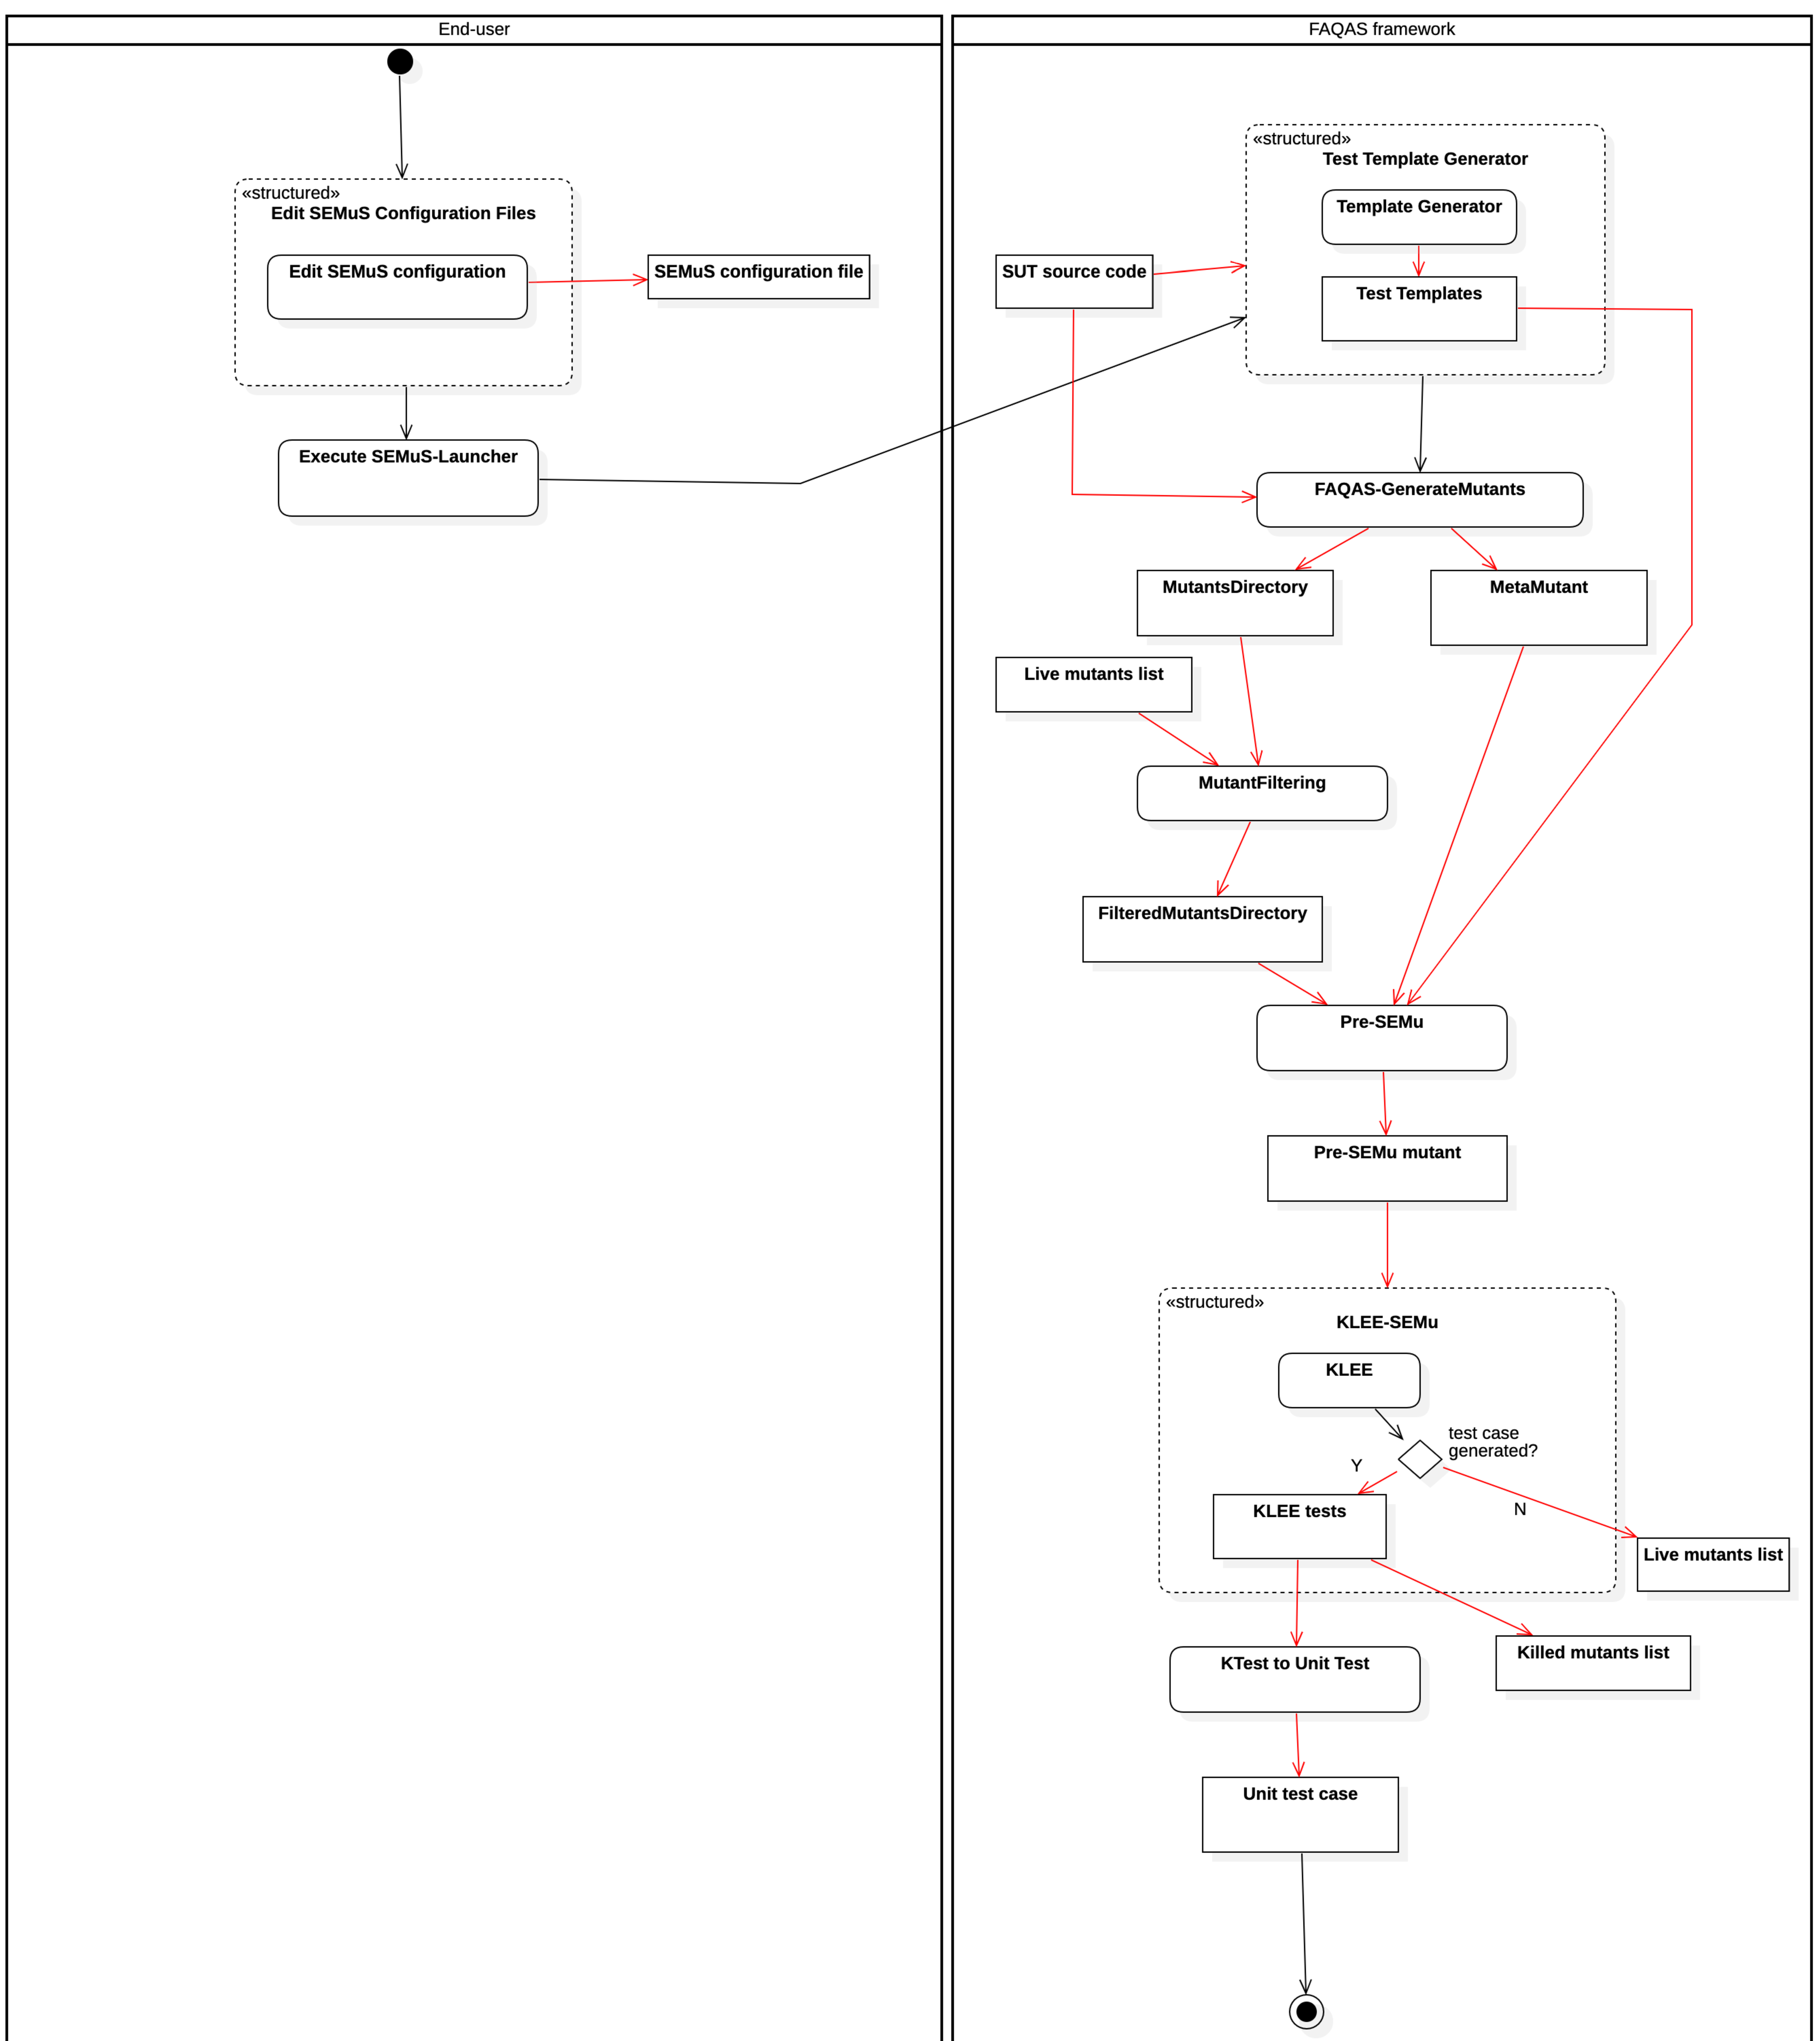
\includegraphics[width=\textwidth]{images/semus-activity.pdf}
  \TODO{Control flow arrows are missing on the SEMUs actor side}
      \caption{Overview of the code-driven test suite augmentation process.}
      \label{fig:process:codeDriven:augmentation}
\end{figure}

SEMuS implements the process for the improvement of the effectiveness of test suites, drafted in Figure~\ref{fig:process:codeDriven:augmentation}. Figure~\ref{fig:process:codeDriven:augmentation} relies on UML activity diagram notation. 
In Figure~\ref{fig:process:codeDriven:augmentation} the execution of specific software artefacts from the end user is made explicit. Also, we use black arrows to draw control-flow, red arrows for data-flow. The activities within the FAQAS Framework swimlane are implemented by a program (i.e., a Python or Bash script) that automates the activity. In the following we introduce a detailed description of the test suite augmentation process.

The activity \emph{Edit SEMuS Configuration} indicates that the engineers must configure the general configuration file; the end-user shall specify the SUT location, source code to be analyzed, and SEMu's specific configurations.

The activity \emph{Template Generator} indicates that SEMuS shall generate the \emph{TestTemplates} based on the SUT source code.
The content of file \emph{TestTemplates} should resemble \emph{Listing 1.23} of D2, it should enable the analysis with KLEE-SEMu. For example, it should have a call to the function targeted by the mutation. Also, it should contain the definition of all the variables used for the execution of KLEE-SEMu and a set of logging functions (e.g., \texttt{printf}) for the returned variable values.

The activity \emph{FAQAS-GenerateMutants} automatically generates a number of copies of each source file, the \emph{MutantsDirectory}, each copy contains one mutant. Additionally to the set mutant's sources, the component generates the \emph{MetaMutant}, which is a C file that embeds all the mutation into one single source file. More details of this activity can be found on Section~\ref{sec:behavior_mass}. 

The activity \emph{MutantFiltering} concerns the filtering of mutants for the test generation process; every mutant that is not present in the list of live mutants is removed from the analysis, and from the \emph{MutantsDirectory}. 

The activity \emph{Pre-SEMu} concerns the generation of a \emph{Pre-SEMu mutant}, that is, a compiled \emph{MetaMutant} file that includes the \emph{TestTemplate} for a specific function under analysis.

The activity \emph{KLEE-SEMu} indicates that SEMuS shall invoke KLEE-SEMu using the \emph{Pre-SEMu mutant} as input, to generate a tentative test input that kills the mutant under analysis. If KLEE-SEMu is not able to generate test inputs for the mutant it will add the identifier of the mutant to a list of live mutants, otherwise the test inputs are stored in the form of KLEE tests and the identifier of the mutant is added to a list of killed mutants.

The activity \emph{KTest To Unit Test} indicates that SEMuS collects the \emph{KLEE tests} generated by \emph{KLEE-SEMu} and generates a readable C unit test case. The test case generated by \emph{KTest to Unit Test} contains an invocation of the function under test (i.e., the function targeted  by the mutation) along with assigned arguments and an assertion that verifies results. The values for the assigned arguments and the verification of results are derived from the output of KLEE.

% The program \emph{FAQAS-GenerateTestGenerationScaffolding} takes as input the path of the \emph{SUT source code} and the file \emph{mutation results csv}. It generates a number of files named \emph{MutantId\_AnalysisMain.c}, one for each live mutant, where MutantId is the ID of a mutant. The file \emph{MutantId\_AnalysisMain.c} contains a main function that should be used for the analysis with KLEE. 



% The activity \emph{Update scaffolding for mutant} in Figure~\ref{fig:process:codeDriven:augmentation} indicates that the engineer should modify the file  \emph{MutantId\_AnalysisMain.c} if necessary. In particular, it might be necessary to refine the assertions produced by \emph{FAQAS-GenerateTestGenerationScaffolding}. More precisely, since assertions should concern output variables, it is necessary to verify that all the necessary output variables had been referred in assertion. Indeed, in C, with pointers and pointers to pointers, it is not possible to have a precise automated identification of output variables.

% The activities in the expansion region \emph{generateTestCase} are repeated for every live mutant.

% The activity \emph{Execute FAQAS-GenerateTestCase} in Figure~\ref{fig:process:codeDriven:augmentation} concerns the execution of the program \emph{FAQAS-GenerateTestCase}.

% The program \emph{FAQAS-GenerateTestCase} generates a tentative unit test case (i.e., a source file in C) that kills the mutant. It executes the KLEE program and then produces a unit test case (i.e., a file with a main in C) after processing the KLEE output.

% For test generation, the support for the programming language of the SUT depends on KLEE (it supports C, limited support for C++).

% The test case generated by \emph{FAQAS-GenerateTestCase} contains an invocation of the function under test (i.e., the function targeted  by the mutation) along with assigned arguments and an assertion that verifies results. The values for the assigned arguments and the verification of results are derived from the output of KLEE.

% If the program \emph{FAQAS-GenerateTestCase} successfully generates a test case, the engineer proceeds with inspecting it (activity \emph{Update Test  Case}), otherwise he can consider the mutant as equivalent (activity \emph{Update mutation results}).

% The activity \emph{Update Test  Case} in Figure~\ref{fig:process:codeDriven:augmentation} is performed by the engineer. He may need to execute the generated test case to verify that KLEE has generated valid inputs (e.g., inputs that meet the program preconditions). Based on KLEE results, \emph{FAQAS-GenerateTestCase} also generates assertions that reflect the output observed by KLEE (e.g., \texttt{assert( output == value\_observed\_by\_KLEE)} ). The engineer should thus also verify that the assertion with the expected value is correct (i.e., it reflects what indicated in the SUT specifications). If the value appearing in the assertion is not correct, it means that KLEE during its execution has observed an incorrect value being generated by the SUT; for this reason, the SUT might be faulty and should be fixed.

% The activity \emph{Add Test Case to SUT Test Suite} in Figure~\ref{fig:process:codeDriven:augmentation} is performed by the engineer, who may add the new test case to the test suite.

% The activity \emph{Update mutation results} in Figure~\ref{fig:process:codeDriven:augmentation} is performed when a test case is not generated. This generally happens when the mutant cannot be killed (i.e., is equivalent). The engineer is expected to manually inspect the mutant to be sure that the mutant is equivalent (otherwise the missing test case is due to a limitation of KLEE). If the mutant is equivalent the engineer removes it from the file \emph{mutation results csv}.

% The activity \emph{Execute FAQAS-RecomputeMutationScore} in Figure~\ref{fig:process:codeDriven:augmentation}  concerns the execution of the program \emph{FAQAS-RecomputeMutationScore}. It is performed after generating test cases for all the live mutants. Program \emph{FAQAS-RecomputeMutationScore} recomputes the mutation score after ignoring the equivalent mutants detected by KLEE.

\subsection{Internal interface design}

All the programs that automate the different steps of SEMuS communicate only through the files that had been described in Section~\ref{sec:component:design:semus}

\subsection{External interface design}

The external interfaces of the SEMuS are the programs that automate the different steps of SEMuS, which have been described above. They are:

\begin{itemize}
  \item \texttt{create\_mutants.sh}: launcher for the generation of mutants.
  \item \texttt{run.sh}: launcher for the generation of test inputs.
  \item \texttt{docker\_run.sh}: launcher for the generation of test inputs by means of Docker.
\end{itemize}








\ENDCHANGEDWPT


\clearpage
\STARTCHANGEDWPT
% !TEX root = MAIN.tex

\section{DAMAt}


\subsection{Software static architecture}

\begin{figure}[h]
  \centering
	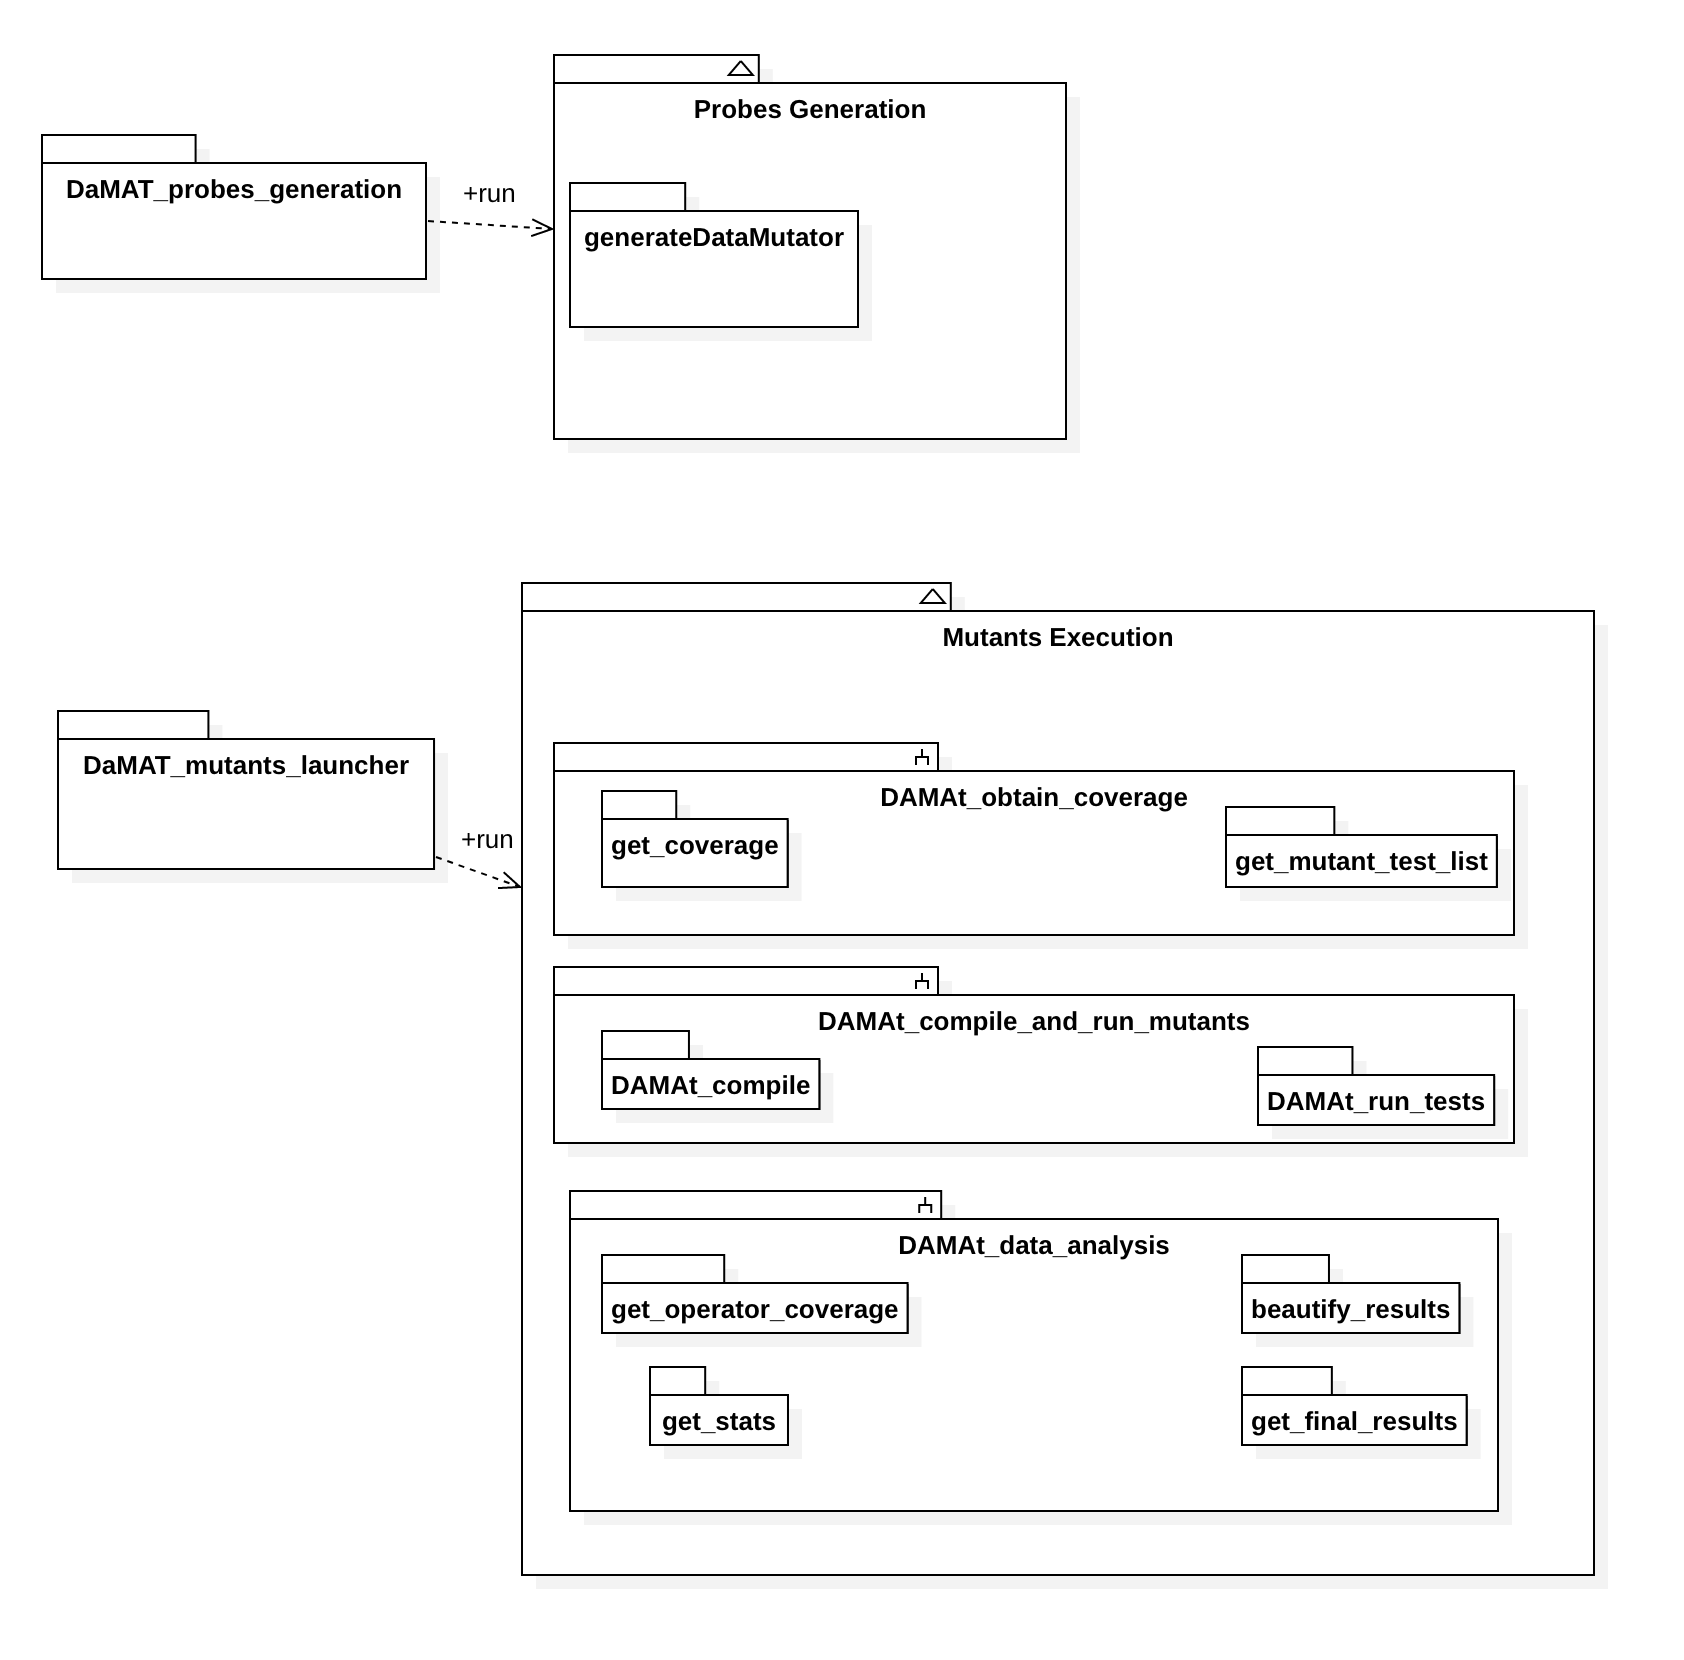
\includegraphics[width=0.8\textwidth]{images/damat_architecture_diagram.png}
      \caption{UML Architecture diagram of \dama.}
      \label{fig:damat_architecture_diagram}
\end{figure}

The architecture of the code-driven mutation analysis toolset (i.e., \dama)  is drafted in
Figure~\ref{fig:damat_architecture_diagram} relying on UML package diagram notation.

As depicted in Figure~\ref{fig:damat_architecture_diagram}, the architecture of the component is divided in two packages, which are named \textit{Probes Generation} and \textit{Mutants Execution} Also, it includes the two entry points:
\begin{itemize}
  \item \textit{damat\_probe\_generation}
  \item \textit{damat\_mutants\_launcher}
\end{itemize}

The package \textit{Probes Generation} implements the features concerning the generation of the data mutation API.

The package \textit{Mutants Execution} implements the features regarding the compilation and execution of mutants, and the analysis of the reusults of the \dama procedure. Note that this layer implements also the strategies for the reduction of the test suite.

\subsubsection{Source Code Structure}


\dama is delivered as a compressed archive consisting of source files.
The following bulletpoints provide a description of the archive's structure once uncompressed:

\begin{itemize}
	\item \textit{damat\_configure.sh}: this script defines the necessary variables for the execution of \dama. They shall be set by the engineer.
	\item \textit{damat\_probe\_generation.sh}: this script set the variables necessary to generate the data mutation API and execute the python script \textit{generateDataMutator.py} to generate them.
	\item \textit{damat\_mutants\_launcher.sh}: this script starts the \dama pipeline.
	\item \textit{generateDataMutator.py}: this is the script that generates the \dama mutation API.
	\item \textit{DDB\_TEMPLATE\_header.c} and \textit{DDB\_TEMPLATE\_footer.c}: these are templates used to generate the \dama API by \textit{generateDataMutator.py}
	\item \textit{damat\_compile.sh}: this is a stub of the script used to compile a mutant, which shall be completed by the engineer.
	\item \textit{damat\_run\_tests.sh}: this is a stub of the script used to run the tests, which shall be completed by the engineer.
	\item \textit{data\_analysis}: a folder containing five python scripts used for the generation of the final results:
	\begin{itemize}
	  \item \textit{beautify\_results.py}: this script renders the raw results from the execution of the tests in a more readable format.
	  \item \textit{get\_coverage.py}: this script analizes the results of the fault model coverage.
	  \item \textit{get\_operator\_coverage.py}: this script analizes the results of the operator coverage.
	  \item \textit{get\_stats.py}: this script produces statistics from the mutants' execution.
		\item \textit{get\_final\_results.py}: this script produces a summary of the execution of \dama.
	\end{itemize}
	\item \textit{pipeline\_scripts}: a folder containing the four scripts that make up the \dama pipeline:
	\begin{itemize}
		\item \textit{damat\_obtain\_coverage.sh}: this script obtains fault model coverage data in order to execute only the tests that cover each mutant.
		\item \textit{get\_mutant\_test\_list.py}: this script produces the list of test against which avery mutant shall be executed.
	  \item \textit{damat\_compile\_and\_run\_mutants.sh}: this scripts compile each mutant and run it against the SUT test suite.
		\item \textit{damat\_data\_analysis.sh}: this script executes all the data analysis steps at the end of the execution of the \dama pipeline
	\end{itemize}
	\item \textit{fault\_model.csv}: an example of a \dama fault model in csv format.
 	\item \textit{tests.csv }: an example of list of test cases and nominal times in csv format.
\end{itemize}
\clearpage

\subsection{Software components design}
\label{sec:damat_component:design}

\begin{figure}[tb]
  \centering
	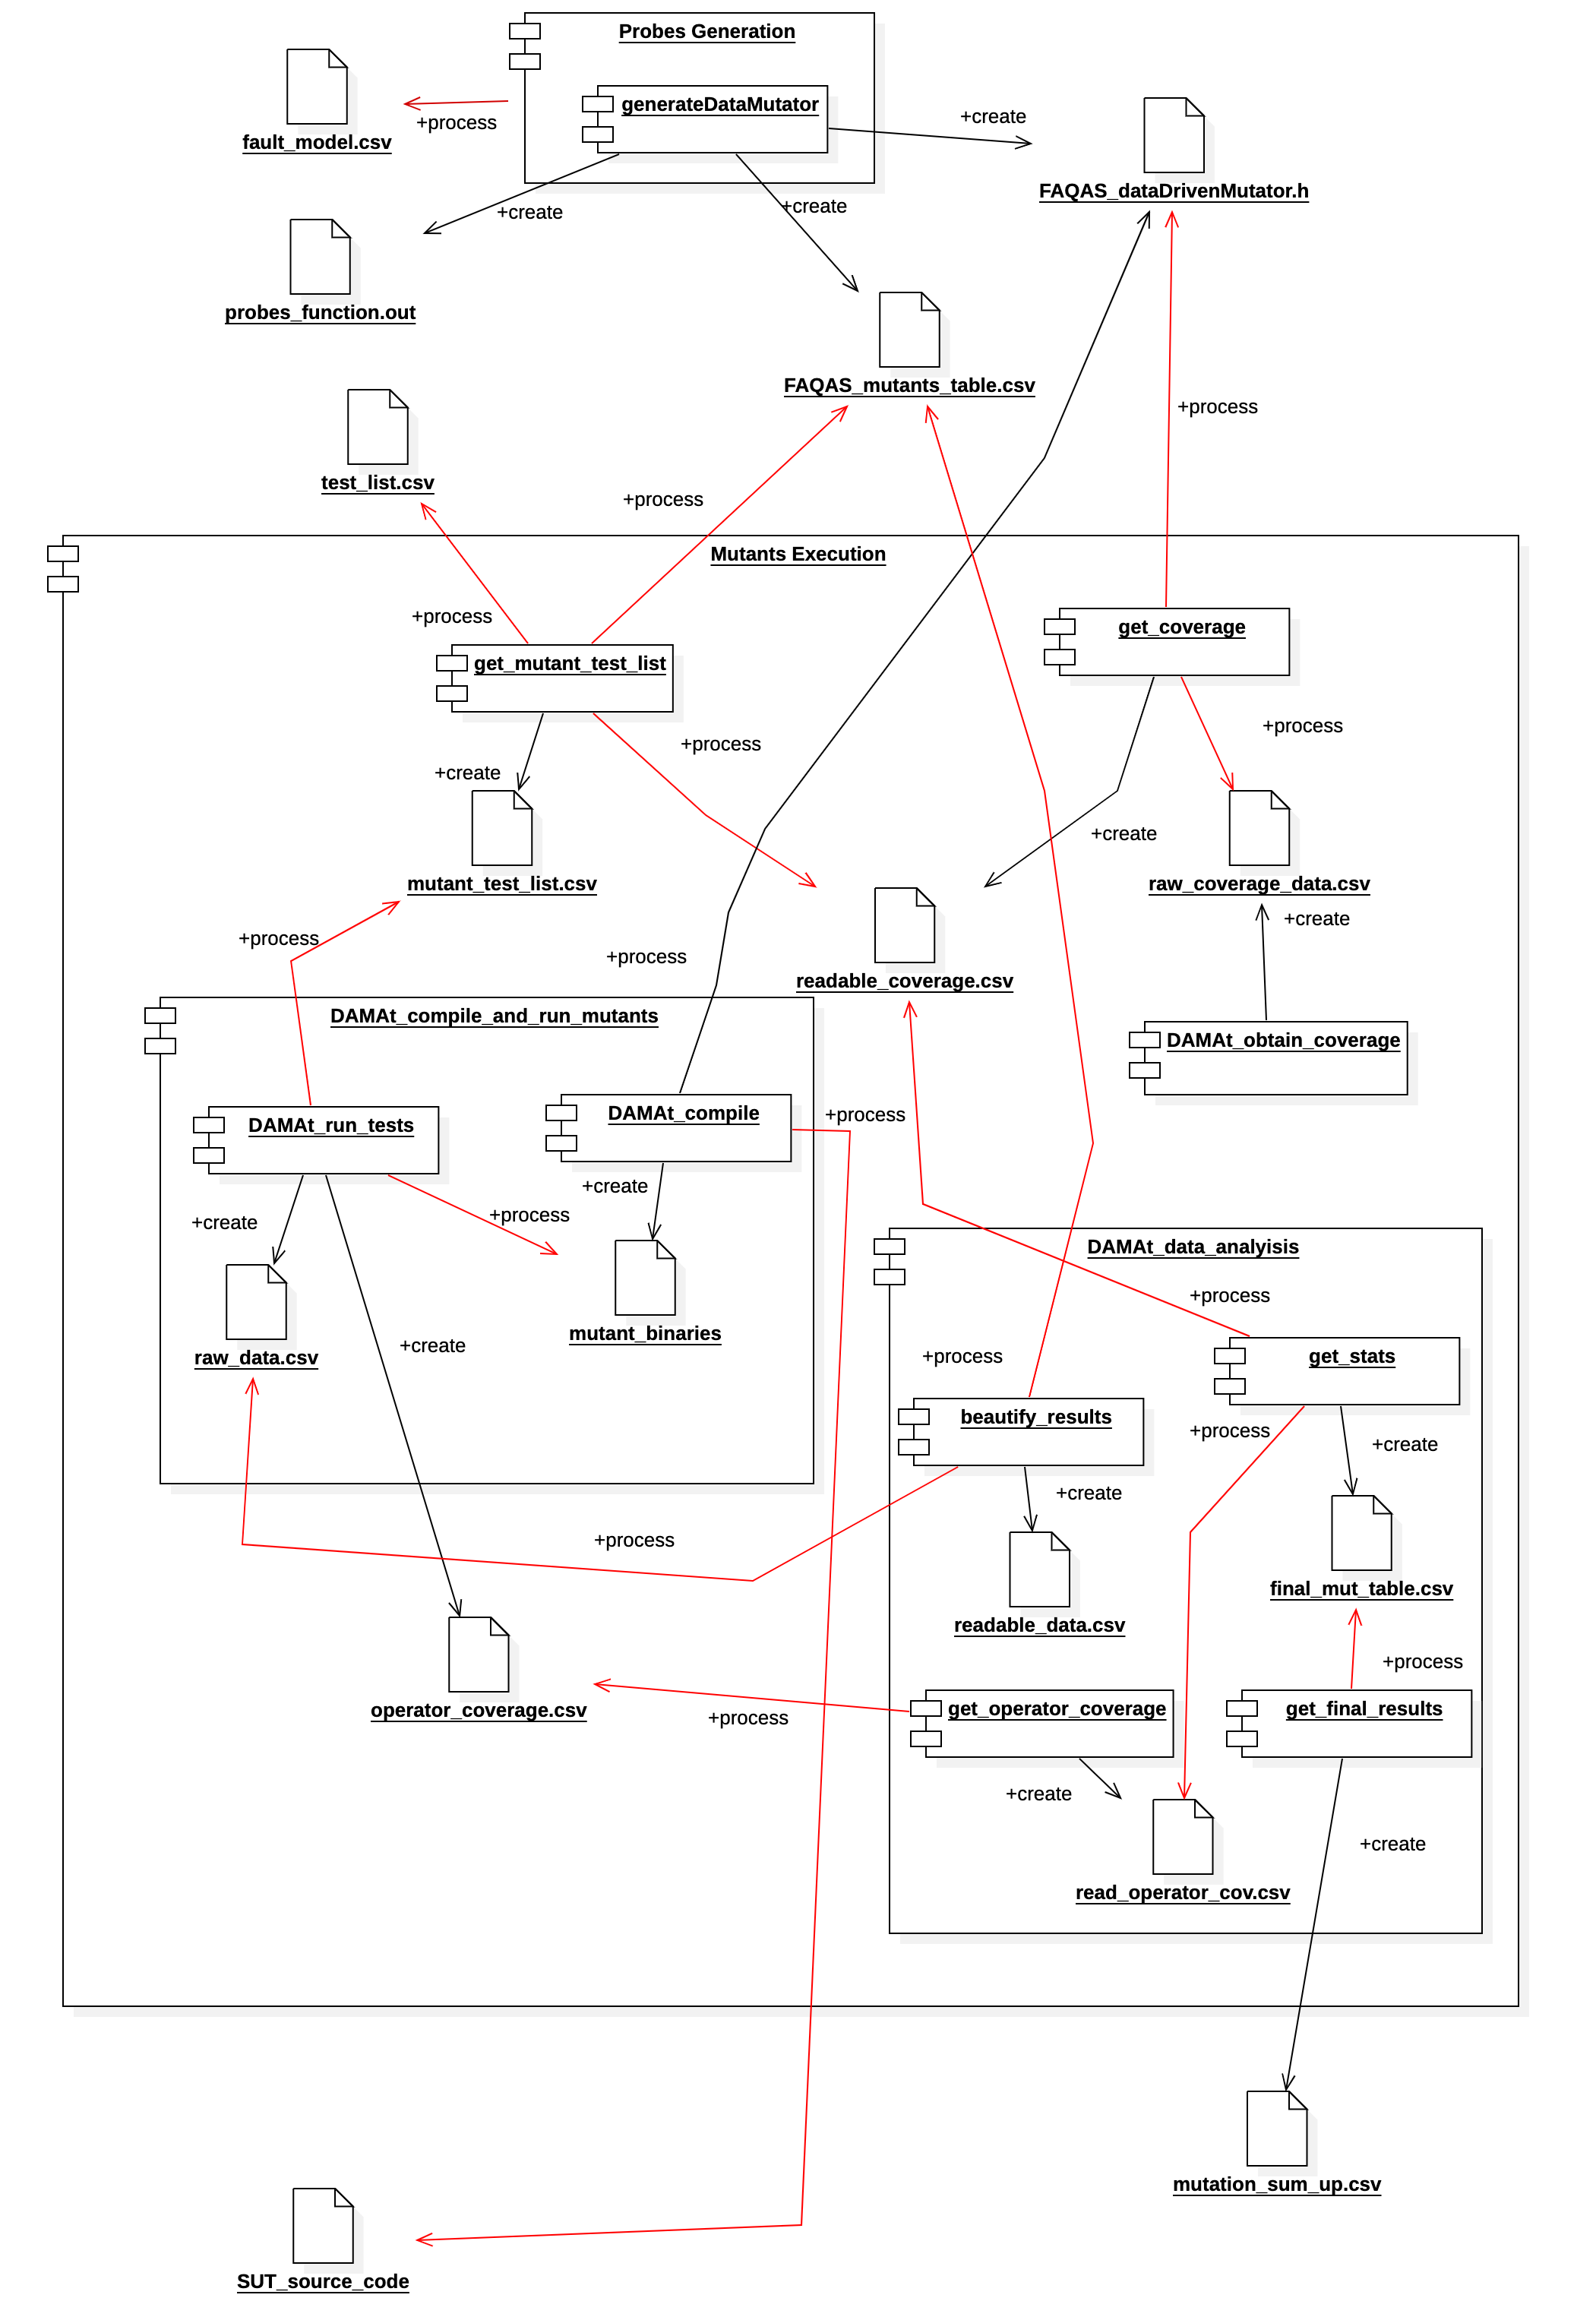
\includegraphics[width=0.9\textwidth]{images/damat_components.png}
      \caption{UML Component diagram of the data-driven mutation testing component to evaluate test suite effectiveness.}
      \label{fig:damat_component_diagram}
\end{figure}

The components of \dama are drafted in Figure~\ref{fig:damat_component_diagram}. Figure~\ref{fig:damat_component_diagram} relies on UML component diagram notation.

As shown in Figure~\ref{fig:damat_component_diagram}, the software is composed by the following components:

\begin{itemize}
  \item \textit{fault\_model.csv}: this csv file shall be provided by the engineer and contains one row per mutation operator. Every mutation operator shall generate one or more mutants.
  For details see D2. An example of line is:

  \texttt{fault\_model\_01,0,1,BIN,BF,3,3,NA,NA,-1,1}

  \item \textit{test\_list.csv}: this csv file shall be provided by the engineer and contains one row per test case, containing an identifier for the test and the mean time of execution expressed in ms. An example of line is:

  \texttt{test\_01,34598}

  \item \textit{Probe  Generation}: this component processes the fault model and and generates \textit{FAQAS\_dataDrivenMutator.h}, \textit{FAQAS\_mutants\_table.csv}  and \textit{probes\_function.out}
  \item \textit{FAQAS\_dataDrivenMutator.h}: this is the API that contains the logic for the data drive mutation.
  \item \textit{FAQAS\_mutants\_table.csv}: this is a csv file containing the definition and \texttt{MutationOpt} (a mumerical ID) for every generated mutant. Every row represents a generated mutant. This is an example of a row:

  \texttt{0,fault\_model\_01,0,1,BIN,BF,3,3,NA,NA,-1,1}

  \item \textit{probes\_function.out}: this file contains prototypes for the mutation probes, which are calls to functions defined in the mutation API.
  \item \textit{Mutants Execution}: this component contains subcomponents that handle the test suite reduction, compilation, execution and data gathering relative to the execution of \dama.
  \begin{itemize}
    \item \textit{DAMAt\_obtain\_coverage}: this component executes a special mutant against the test suite that collects the \textit{raw\_coverage\_data.csv} file.

    \item \textit{raw\_coverage\_data.csv}: this file is a collection of the coverage data for each test. A row is produced every time a mutation function is called. It contains a numerical ID realtive to the fault model.
    This is an example of row:

    \texttt{fm.ID: 0}

    \item \textit{get\_coverage}: this component process the \textit{raw\_coverage\_data.csv} file to produce \textit{readable\_coverage\_data.csv}.

    \item \textit{readable\_coverage\_data.csv}: this file is a collection of the coverage data for each couple test-fault model in a more accessible and compact format.
    This is an example of row:

    \texttt{test\_01,fault\_model\_01,<coverage status>,<nr of calls>}

    \item \textit{get\_mutant\_test\_list}: this component processes \textit{test\_list.csv} and \textit{readable\_coverage\_data.csv} to produce \textit{mutant\_test\_list.csv}.

    \item \textit{mutant\_test\_list.csv} is a csv file containing a reduced version of \textit{test\_list.csv} specific for every mutant with only the tests covering that specific mutant. The structure is the same as \textit{test\_list.csv}.

    \item \textit{DAMAt\_compile\_and\_run\_mutants}: this component contains subcomponents that compile the generated mutants and run them against the test suite of the SUT.
    \begin{itemize}
      \item \textit{DaMAT\_compile}: this component processes \textit{FAQAS\_dataDrivenMutator.h} and the \textit{SUT source code} to produce the \textit{mutant binary files}.
      \item \textit{DAMAt\_run\_tests}: this component processes the \textit{mutant binary files} and the \textit{mutant\_test\_list.csv}, producing \textit{raw\_data.csv} and \textit{operator\_coverage.csv}.
      \item \textit{raw\_data.csv} is a file in the csv format. Each row contains the result of the execution of a mutant against a test case.
      This is an example:

      \begin{lstlisting}
      <mutationOpt>;COMPILED;test_01;PASSED;LIVE;<elapsed time>
      <mutationOpt>;COMPILED;test_02;FAILED;KILLED;<elapsed time>
      \end{lstlisting}

      \item \textit{operator\_coverage.csv}: this is a file in the csv format. Every row describes a call to the mutation API. The firs column contains an sequential index that identifies the call and the second row contains \texttt{1} if the mutation operator was successfully applied or \texttt{0} if not.
      This is an example or a row:

      \texttt{234,0}

    \end{itemize}
    \item \textit{DAMAt\_data\_analysis}: this component contains subcomponents that analise the data produced from an execution of \dama and produce the final results.
    \begin{itemize}
      \item \textit{beautify\_results}: this component processes \textit{raw\_data.csv} and \textit{FAQAS\_mutants\_table.csv} to produce \textit{readable\_data.csv}
      \item \textit{readable\_data.csv} is a more complete csv. Every row represents a mutant-test case couple and contains the definition of the mutant.
      An example is provided below:

      \begin{lstlisting}
      <mutationOpt>,COMPILED,test_01,PASSED,LIVE,36378,fault_model_01,0,1,BIN,BF,3,3,NA,NA,-1,1
      <mutationOpt>,COMPILED,test_02,PASSED,LIVE,43364,fault_model_02,28,2,DOUBLE,VOR,-20,50,NA,1,NA,NA
      \end{lstlisting}

      \item \textit{get\_operator\_coverage} this component processes  \textit{operator\_coverage.csv} to produce \textit{readable\_operator\_coverage.csv}
      \item \textit{readable\_operator\_coverage.csv}: this cvs file is a rendition of /\textit{operator\_coverage.csv} in a more compact and undertandable format.
      every row represent a mutant-test case couple. the srtucture is provoded below

      \texttt{<MutationOpt>,<testID>,<nr of calls>,<number of successful application>}

      \item \textit{get\_stats} this component processes \textit{readable\_coverage.csv}, \textit{readable\_operator\_coverage.csv} and \textit{readable\_data.csv} to produce \textit{final\_mutants\_table.csv}
      \item \textit{final\_mutants\_table.csv} is a file in the csv format that contains a row for every mutant. Every row contains informations about the mutant definition and status.
      An example is provided below:

      \begin{lstlisting}
      <MutationOpt>,fault_model_01,0,1,BIN,BF,3,3,NA,NA,-1,1,LIVE,APPLIED
      <MutationOpt>,fault_model_02,0,1,BIN,BF,4,4,NA,NA,-1,1,NOT_COVERED,NOT_APPLIED
      \end{lstlisting}

      \item \textit{get\_final\_results}: this component processes \textit{final\_mutants\_table.csv} to produce \textit{mutation\_sum\_up.csv}
      \item \textit{mutation\_sum\_up.csv} is a csv file that contains a summary of the execution of \dama.
      An example is provided below:

      \begin{lstlisting}
      all_fault_models,covered_fault_models,fault_model_coverage
      11,2,0.182
      covered_mutants,applied_mutants,operator_coverage
      2,2,1.0
      applied_mutants,killed_mutants,mutation_score
      2,0,0.0
      \end{lstlisting}

    \end{itemize}
  \end{itemize}

\end{itemize}
\clearpage


% \begin{figure}[h]
%   \centering
% 	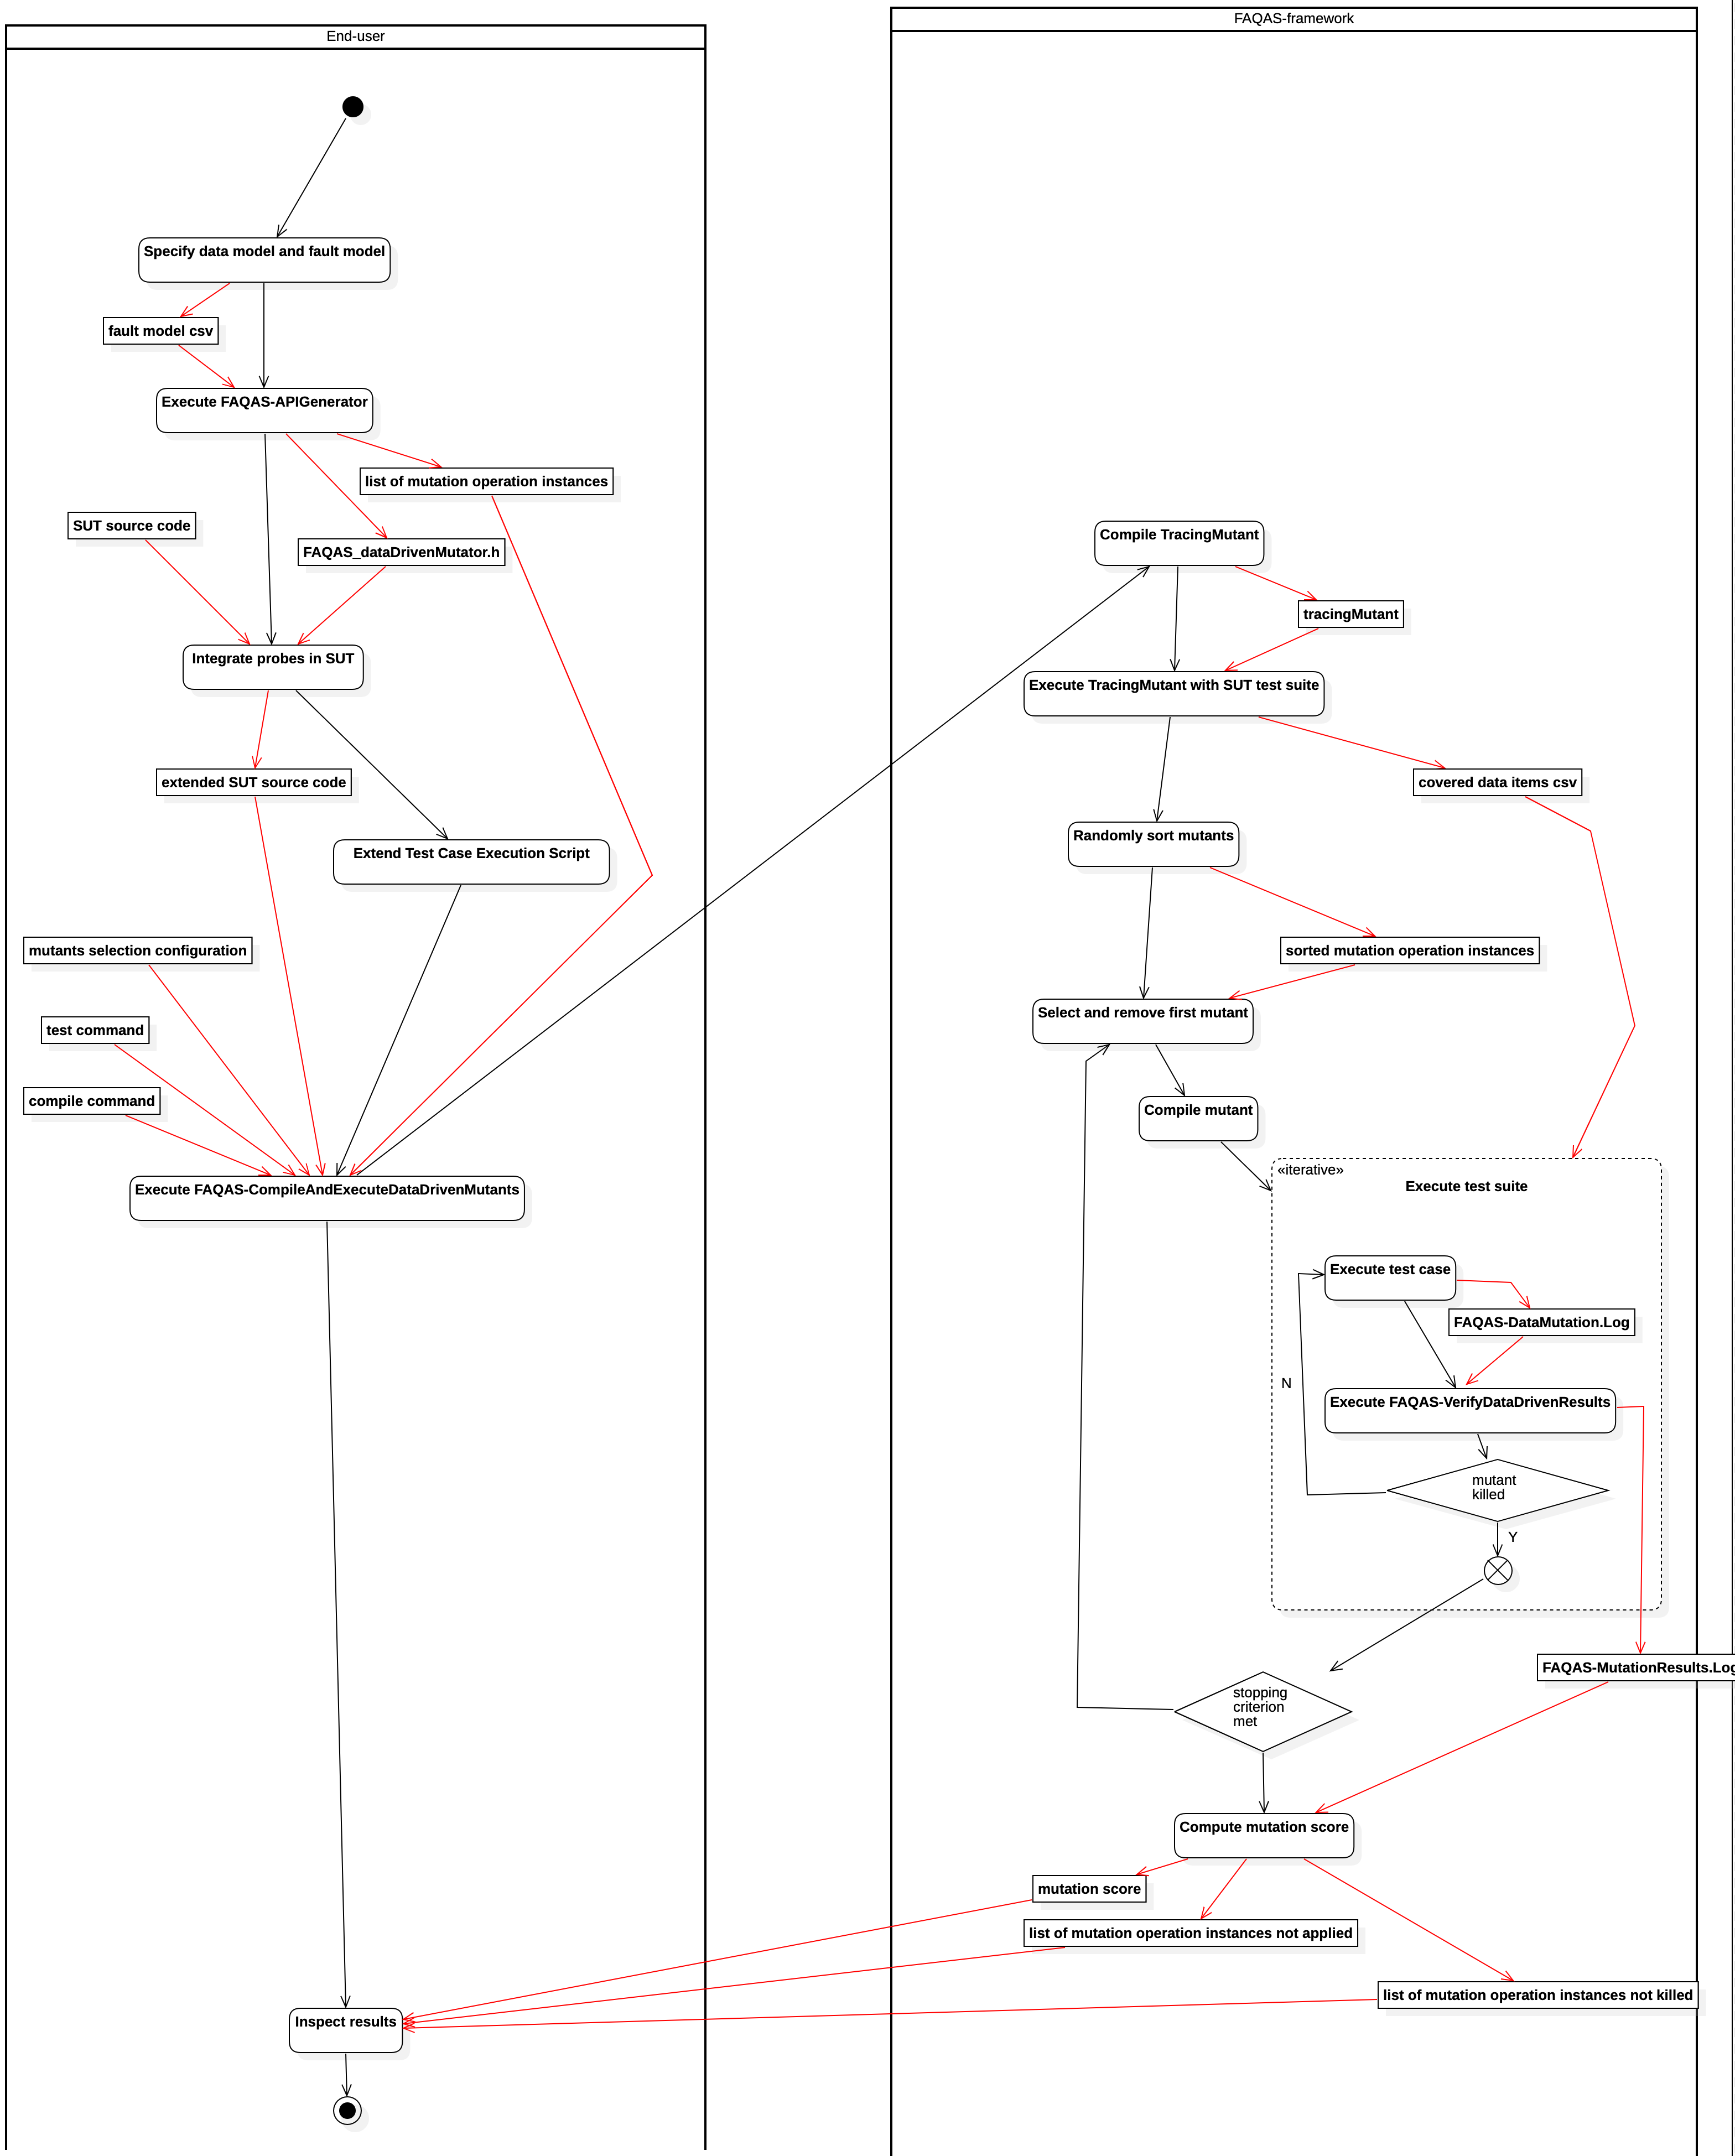
\includegraphics[width=\textwidth]{images/png/Activity1!DataDrivenTestSuiteEvaluation_3.png}
%       \caption{Overview of the data-driven mutation testing process to evaluate test suite effectiveness.}
%       \label{fig:process:dataDriven:evaluation}
% \end{figure}
%
% The data-driven mutation testing component shall implement the process for the evaluation of test suite effectiveness that is drafted in Figure~\ref{fig:process:dataDriven:evaluation}. Figure~\ref{fig:process:dataDriven:evaluation} relies on UML activity diagram notation. In Figure~\ref{fig:process:dataDriven:evaluation} the execution of specific software artefacts by the end-user is made explicit. Also, we use black arrows to draw control-flow, red arrows for data-flow.
%
% The activity \emph{Specify data model and fault model} in Figure~\ref{fig:process:dataDriven:evaluation} indicates that the engineer should prepare a csv file specifying the fault model and the data model for the SUT according to D2.
%
% The activity \emph{Execute FAQAS-APIGenerator} in Figure~\ref{fig:process:dataDriven:evaluation} concerns the execution of the program \emph{Execute FAQAS-APIGenerator}.
%
% The program \emph{FAQAS-APIGenerator} takes as input the \emph{fault model csv} and generates the file \emph{FAQAS\_dataDrivenMutator.h} and a csv file containing the \emph{list of mutation operation instances} derived from the fault model.
%
% File \emph{FAQAS\_dataDrivenMutator.h} contains the FAQAS mutation testing API (i.e., the predefined functions to perform data mutation for buffers) and the fault model represented as a data structure. Details are provided in D2.
%
% The activity \emph{Integrate probes in SUT} in Figure~\ref{fig:process:dataDriven:evaluation} indicates that the engineer should manually modify the source code of the SUT to integrate mutation probes into it. Examples are provided in \emph{Listing 2.3}, \emph{Listing 3.1}, and \emph{Appendix A - Section 1.1} of D2.
%
% The activity \emph{Extend Test Case Execution Script} in Figure~\ref{fig:process:dataDriven:evaluation} indicates that the engineer is expected to manually modify the scripts used to execute test cases so that they include an invocation to \emph{FAQAS-VerifyDataDrivenResults} after the execution of every single test case.
%
% The activity \emph{Execute FAQAS-CompileAndExecuteDataDrivenMutants} in Figure~\ref{fig:process:dataDriven:evaluation} concerns the execution of the program \emph{Execute FAQAS-CompileAndExecuteDataDrivenMutants}.
%
% The program \emph{Execute FAQAS-CompileAndExecuteDataDrivenMutants} receives as inputs the command to compile the SUT, the command to execute the test suite, the path to the extended SUT source code, and the mutants selection configuration. It automatically executes a number of activities required to compute the mutation score: \emph{Compile TracingMutant}, \emph{Execute TracingMutant with SUT test suite}, \emph{Randomly sort mutants}, \emph{Select and remove first mutant}, \emph{Compile mutant}, \emph{Execute test suite},  \emph{Compute mutation score}.
%
% The program \emph{FAQAS-CompileAndExecuteDataDrivenMutants} implements the four mutants selection strategies: \emph{all mutants} (i.e., all the mutants are tested), \emph{proportional uniform sampling} (i.e., a subset of the mutants is tested selected based on a percentage), \emph{uniform fixed-size sampling} (i.e., a subset of the mutants is tested selected based on a fixed number), and \emph{uniform FSCI sampling} (i.e., a subset of the mutants is tested, they are selected according to the FSCI criterion).
%
% The \emph{mutants selection configuration} indicates the mutants selection strategy and a configuration value that specifies the number of mutants to consider; the value may indicate the percentage of mutants to sample (for \emph{proportional uniform sampling}), the number of mutants to sample (for \emph{uniform fixed-size sampling}), or the size of the confidence interval (for \emph{uniform FSCI sampling}).
%
% The activity \emph{Compile TracingMutant} indicates that the system compiles a version of the SUT that traces the data items (targeted by mutation) that are covered by each test case (see D2, Figure 2.9, line 5).
%
% The activity \emph{Execute TracingMutant with SUT test suite} indicates that the system executes the SUT test suite. Since the test suite is executed with the TracingMutant it leads to the generation of a csv files that indicates, for every test case, the data items being exercised by the test case.
%
% The activity \emph{Randomly sort mutants} indicates that  \emph{FAQAS-CompileAndExecuteDataDrivenMutants} generates a randomly sorted list of mutation operation instances. This list is derived from the \emph{list of mutation operation instances}.
%
% The activity \emph{Select and remove first mutant} indicates that  \emph{FAQAS-CompileAndExecuteMutants} selects the first item in the \emph{sorted mutation operation instances} and removes it from the list.
%
% The activity \emph{Compile mutant} indicates that the system compiles a version of the SUT with the selected mutation operation instance enabled.
%
% The activity \emph{Execute test case} indicates that the test suite of the SUT executes a test case. Only the test cases exercising the data item targeted by the mutation operator are executed. Since the test case is executed against the mutated SUT, if the mutation operation is performed, then the file \emph{FAQAS-MutationResults.Log} will be created (this is a feature of the FAQAS data-driven mutation API).
%
% File \emph{FAQAS-MutationResults.Log} contains the ID of the mutation operation instance applied.
%
% Program \emph{FAQAS-VerifyDataDrivenResults} receives as input the ID of the test case and  the status of a test case (i.e., PASS or FAIL). It checks if a data mutation operator has been applied based on the content of \emph{FAQAS-DataMutation.Log}. It deletes \emph{FAQAS-DataMutation.Log}. It updates the content of \emph{FAQAS-MutationResults.Log}.
%
% If program \emph{FAQAS-VerifyDataDrivenResults} determines that a mutation operation instance has been killed, then the test suite execution is terminated.
%
% File \emph{FAQAS-MutationResults.Log} indicates, for every executed test case, the ID of the mutation operation instance applied and the mutation result (KILLED or LIVE). A test case may appear multiple times in this file, each time with a different mutation operation instance ID associated.
%
% The execution of the test suite is repeated till a termination criterion is met. The termination criterion depends on the mutants selection strategy:
% \begin{itemize}
% \item \emph{all mutants}: the list \emph{sorted list of mutants} is empty
% \item \emph{proportional uniform sampling}: a number of mutants matching the selected percentage has been executed
% \item \emph{uniform fixed-size sampling}: a number of mutants matching the selected value has been executed
% \item \emph{uniform FSCI sampling}: the confidence interval computed from \emph{mutation results csv} is smaller than the length specified by the user.
% \end{itemize}
%
% The activity \emph{Compile mutation score} concerns the computation of the mutation score based on the mutation results reported in \emph{FAQAS-MutationResults.Log}. The formula is provided in D2. As output of the computation of the mutation score the system reports also the \emph{list of mutation operation instances not killed} and the \emph{list of mutation operation instances not applied}. The \emph{list of mutation operation instances not killed} includes also the name of test cases executed for each, to facilitate the improvement of the test suite.
%
% The end-user inspects the \emph{list of mutation operation instances not applied} to understand which data types had not been covered by the test suite. The end-user inspects the \emph{list of mutation operation instances not killed} to understand which test cases need improvement.

\ENDCHANGEDWPT
%

\clearpage
% !TEX root = MAIN.tex


\subsection{Data-Driven Test Suite Augmentation}

\begin{figure}[]
  \centering
	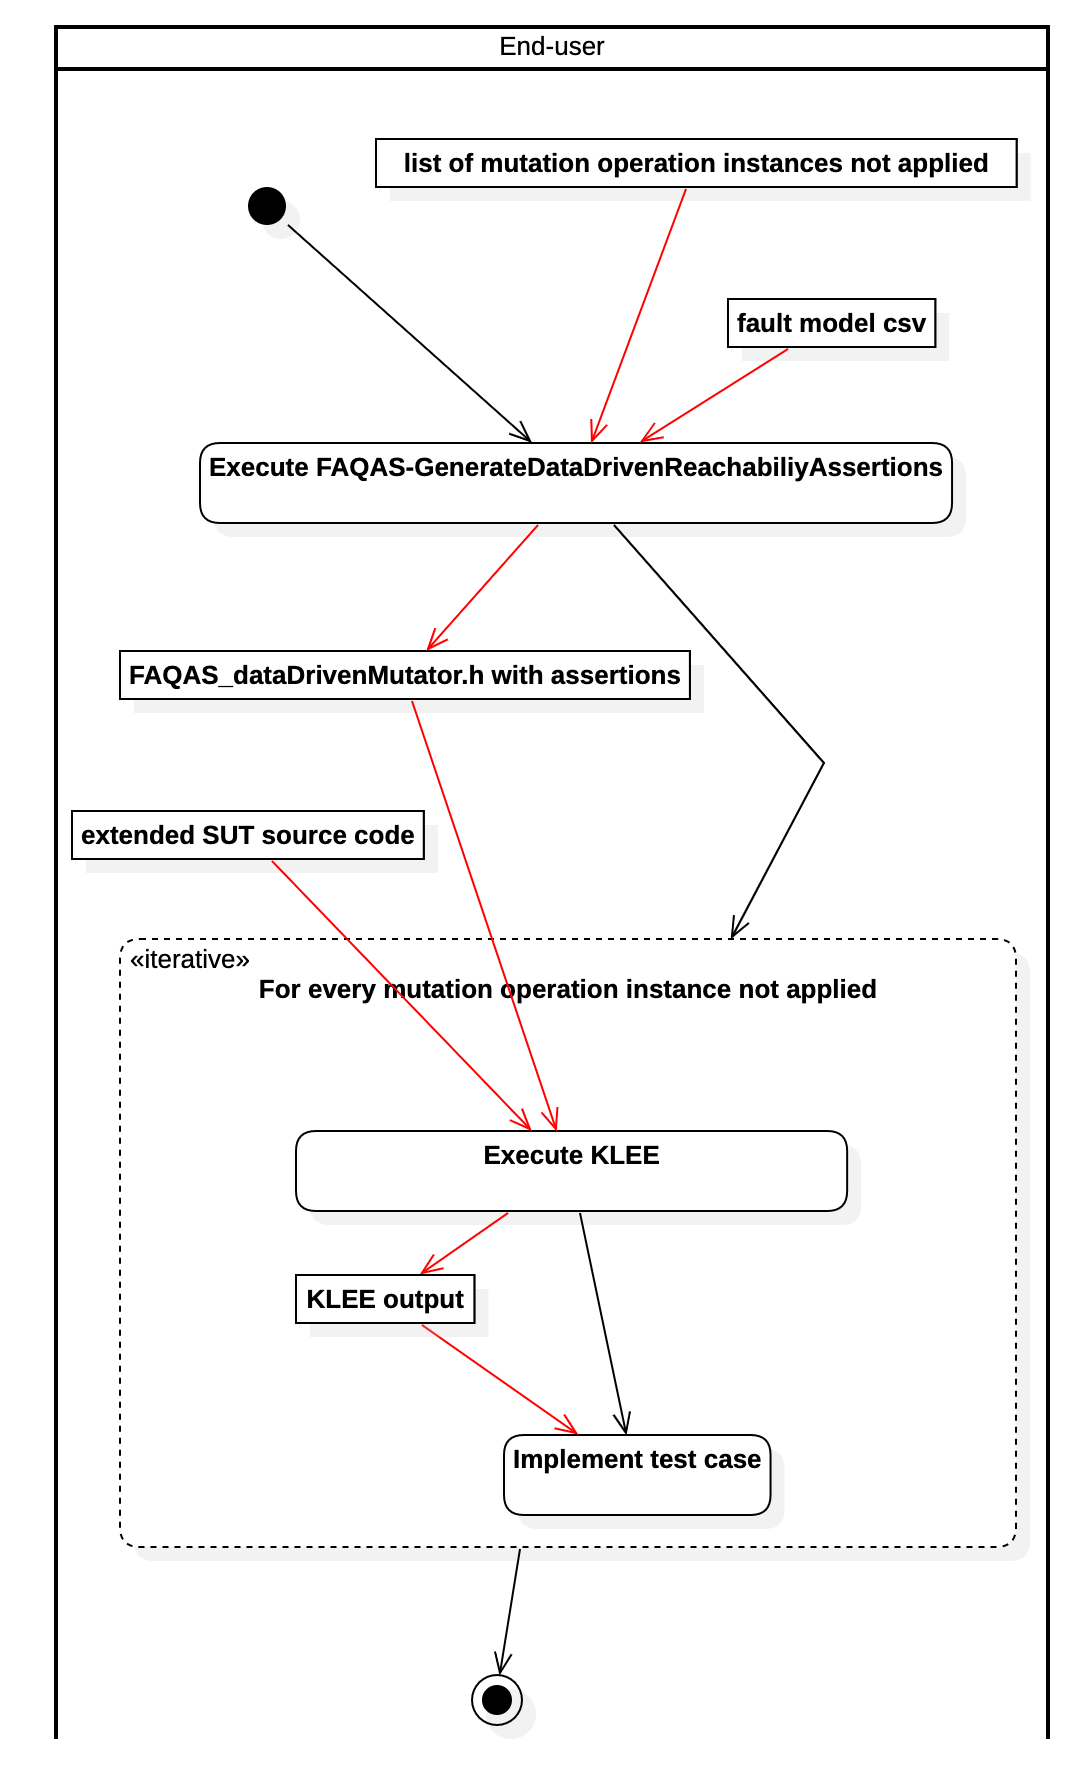
\includegraphics[width=0.4\textwidth]{images/png/Activity1!DataDrivenTestSuiteAugmentation_4.png}
      \caption{Overview of the data-driven test suite augmentation process.}
      \label{fig:process:dataDriven:augment}
\end{figure}

The activity \emph{Execute FAQAS-GenerateDataDrivenReachabiliyAssertions} in Figure~\ref{fig:process:dataDriven:augment} concerns the execution of the program \emph{Execute FAQAS-GenerateDataDrivenReachabiliyAssertions}.

The program \emph{FAQAS-GenerateDataDrivenReachabiliyAssertions} takes as input the fault model and generates a version of \emph{FAQAS\_dataDrivenMutator.h} that contains reachability assertions that enable KLEE to generate inputs that reach the mutation.

The activity \emph{Execute KLEE} indicates that the end-user should execute KLEE, after performing the required scaffolding, if necessary. A methodological procedure document to support the end-user will be provided.

The activity \emph{Implement test case} indicates that the end-user should implement a test case based on KLEE's output.



% % !TEX root = MAIN.tex

\chapter{MASS - Software Unit Test Case Design}


\section{General}

The MASS unit test suite concerns the source code mutation component (SRCMutation). It address its functional requirements. A single test design has been identified: it is based on the category partition method and reported in the following sections.



\section{MASS - Test Design - SRCMutation - Operators}

\subsection{Test design identifier}

The test design identifier is \emph{MASS-TD-SRCMutation-1}

With this test design we aim to ensure that each mutation operator for the \FAQAS is implemented according to its requirements.

\subsection{Features to be tested}

Table~\ref{table:operators} shows the specifications for the mutation operators implemented by SRCMutation.

The set of SRCMutation mutation operators is composed of the following: Absolute Value Insertion (ABS), Arithmetic Operator Replacement (AOR), Integer Constraint Replacement (ICR), Logical Connector Replacement (LCR), Relational Operator Replacement (ROR), Unary Operator Insertion (UOI), Statement Deletion Operator (SDL), and Literal Value Replacement (LVR).
It also includes OODL mutation operators: delete Arithmetic (AOD), Bitwise (BOD), Logical (LOD), Relational (ROD), and Shift (SOD) operators.

% !TEX root =  ../Main.tex

\newcommand{\op}{\mathit{op}}
\newcommand{\ArithmeticSet}{ \texttt{+}, \texttt{-}, \texttt{*}, \texttt{/}, \texttt{\%} }
\newcommand{\LogicalSet}{ \texttt{&&}, \texttt{||} }
\newcommand{\RelationalSet}{ \texttt{>}, \texttt{>=}, \texttt{<}, \texttt{<=}, \texttt{==}, \texttt{!=} }
\newcommand{\BitWiseSet}{ \texttt{\&}, \texttt{|}, \land }
\newcommand{\ShiftSet}{ \texttt{>>}, \texttt{<<} }


\begin{table}[h]
\caption{Implemented set of mutation operators.}
\label{table:operators} 
\centering
\scriptsize
\begin{tabular}{|@{}p{4mm}@{}|@{}p{2cm}@{\hspace{1pt}}|@{}p{11.1cm}@{}|}
\hline
&\textbf{Operator} & \textbf{Description$^{*}$} \\
\hline
\multirow{7}{*}{\rotatebox{90}{\emph{Sufficient Set}}}&ABS               & $\{(v, -v)\}$	\\
\cline{2-3}
&AOR               & $\{(\op_1, op_2) \,|\, \op_1, \op_2 \in \{ \ArithmeticSet \} \land \op_1 \neq \op_2 \} $       \\
&    			  & $\{(\op_1, \op_2) \,|\, \op_1, \op_2 \in \{\texttt{+=}, \texttt{-=}, \texttt{*=}, \texttt{/=}, \texttt{\%} \texttt{=}\} \land \op_1 \neq \op_2 \} $       \\
\cline{2-3}
&ICR               & $\{i, x) \,|\, x \in \{1, -1, 0, i + 1, i - 1, -i\}\}$           \\
\cline{2-3}
&LCR               & $\{(\op_1, \op_2) \,|\, \op_1, \op_2 \in \{ \texttt{\&\&}, || \} \land \op_1 \neq \op_2 \}$            \\
&				  & $\{(\op_1, \op_2) \,|\, \op_1, \op_2 \in \{ \texttt{\&=}, \texttt{|=}, \texttt{\&=}\} \land \op_1 \neq \op_2 \}$            \\
&				  & $\{(\op_1, \op_2) \,|\, \op_1, \op_2 \in \{ \texttt{\&}, \texttt{|}, \texttt{\&\&}\} \land \op_1 \neq \op_2 \}$            \\
\cline{2-3}
&ROR               & $\{(\op_1, \op_2) \,|\, \op_1, \op_2 \in \{ \RelationalSet \}\}$            \\
&				  & $\{ (e, !(e)) \,|\, e \in \{\texttt{if(e)}, \texttt{while(e)}\} \}$ \\
\cline{2-3}
&SDL               & $\{(s, \texttt{remove}(s))\}$            \\
\cline{2-3}
&UOI               & $\{ (v, \texttt{--}v), (v, v\texttt{--}), (v, \texttt{++}v), (v, v\texttt{++}) \}$            \\   
\hline
\hline
\multirow{5}{*}{\rotatebox{90}{\emph{OODL}}}&AOD               & $\{((t_1\,op\,t_2), t_1), ((t_1\,op\,t_2), t_2) \,|\, op \in \{ \ArithmeticSet \} $       \\ 
\cline{2-3}
&LOD               & $\{((t_1\,op\,t_2), t_1), ((t_1\,op\,t_2), t_2) \,|\, op \in \{  \} \}$       \\ 
\cline{2-3}
&ROD               & $\{((t_1\,op\,t_2), t_1), ((t_1\,op\,t_2), t_2) \,|\, op \in \{ \RelationalSet \} \}$       \\ 
\cline{2-3}
&BOD               & $\{((t_1\,op\,t_2), t_1), ((t_1\,op\,t_2), t_2) \,|\, op \in \{ \BitWiseSet \} \}$       \\ 
\cline{2-3}
&SOD               & $\{((t_1\,op\,t_2), t_1), ((t_1\,op\,t_2), t_2) \,|\, op \in \{ \ShiftSet \} \}$       \\ 
%\hline
%COR               & $\{(\op_1, \op_2) \,|\, \op_1, \op_2 \in \{ \texttt{\&\&}, \texttt{||}, \land \} \land \op_1 \neq \op_2 \}$            \\
\hline
\hline
\multirow{3}{*}{\rotatebox{90}{\emph{Other}}}&LVR			& $\{(l_1, l_2) \,|\, (l_1, l_2) \in \{(0,-1), (l_1,-l_1), (l_1, 0), (\mathit{true}, \mathit{false}), (\mathit{false}, \mathit{true})\}\}$\\
&&\\
&&\\
\hline
\end{tabular}

$^{*}$Each pair in parenthesis shows how a program element is modified by the mutation operator. Th eleft element of the pair is replaced with the right element. We follow standard syntax~\cite{kintis2018effective}. Program elements are literals ($l$), integer literals ($i$), boolean expressions ($e$), operators ($\op$), statements ($s$), variables ($v$), and terms ( $t_i$, which might be either variables or literals).
\end{table}



Each mutation operator, when applied to a statement, generates one or more mutated statements by altering the value of a \emph{term} in a statement, which could be either an operator  ($op$), a value ($v$), or a literal ($l$). More precisely, each mutation operator  replaces a term with a number of replacement terms, which are identified following the rules in the description column of Table~\ref{table:operators}.
For each term to mutate, SRCMutation shall generate one mutant for every replacement term contained in its description.
If a statement includes more than one term to mutate, the mutation operator generates a set of mutants for each term to mutate. Table~\ref{table:operators:terms}, shows, for every mutation operator the terms it targets and the replacement terms (separated by comma). Replacement terms shall be used when defining test assertions (i.e., we shall verify that the term to mutate has been replaced any of the available replacements, one for each generated mutant).


% !TEX root =  ../MAIN.tex

\begin{table}[h]
\scriptsize
\centering
\caption{Terms to mutate and replacements per mutation oprator.}
\label{table:operators:terms}

\begin{tabular}{lll}
\hline 
\textbf{Operator}	&	\textbf{Term to mutate}	&	\textbf{Replacements}\\
\hline 
ABS	&	$v$	&	$-v$	\\
AOR	&	$+$	&	$ -,*,/,\% $	\\
AOR	&	$-$	&	$ +,*,/,\% $	\\
AOR	&	$*$	&	$ +,-,/,\% $	\\
AOR	&	$/$	&	$ +,-,*,\% $	\\
AOR	&	$\%$	&	$ +,-,*,/ $	\\
AOR	&	$+=$	&	$ -=,*=,/=,\%= $	\\
AOR	&	$-=$	&	$ +=,*=,/=,\%= $	\\
AOR	&	$*=$	&	$ +=,-=,/=,\%= $	\\
AOR	&	$/=$	&	$ +=,-=,*=,\%= $	\\
AOR	&	$\%=$	&	$ +=,-=,*=,/= $	\\
ICR	&	$i$	&	$ 1, -1, 0, i+1, i-1, -i $	\\
LCR	&	$\&\&$	&	$||$	\\
LCR	&	$||$	&	$\&\&$	\\
LCR	&	$\&$	&	$ |,\land $	\\
LCR	&	$|$	&	$ \&,\land $	\\
LCR	&	$\land$	&	$ \&,| $	\\
LCR	&	$\&=$	&	$ |=, \land= $	\\
LCR	&	$|=$	&	$ \&=, \land= $	\\
LCR	&	$\land=$	&	$ \&=, |= $	\\
ROR	&	$>$	&	$ >=, <, <=, ==, != $	\\
ROR	&	$>=$	&	$ >, <, <=, ==, != $	\\
ROR	&	$<$	&	$ >, >=, <=, ==, != $	\\
ROR	&	$<=$	&	$ >, >=, <, ==, != $	\\
ROR	&	$==$	&	$ >, >=, <, <=, != $	\\
ROR	&	$!=$	&	$ >, >=, <, <=, == $	\\
ROR	&	\texttt{if(e )}	&	\texttt{if(!e)}	\\
ROR	&	\texttt{while( e)}	&	\texttt{while(!e)}	\\
SDL	&	$s$	&	\texttt{remove(s)}	\\
UOI	&	$v$	&	$ \texttt{--}v, v\texttt{--}, \texttt{++}v, v\texttt{++} $	\\
AOD	&	$a + b$	&	$ a, b $	\\
AOD	&	$a - b$	&	$ a, b $	\\
AOD	&	$a * b$	&	$ a, b $	\\
AOD	&	$a / b$	&	$ a, b $	\\
AOD	&	$a \% b$	&	$ a, b $	\\
LOD	&	$a \&\& b$	&	$ a, b $	\\
LOD	&	$a || b$	&	$ a, b $	\\
ROD	&	$>$	&	$ a, b $	\\
ROD	&	$>=$	&	$ a, b $	\\
ROD	&	$<$	&	$ a, b $	\\
ROD	&	$<=$	&	$ a, b $	\\
ROD	&	$==$	&	$ a, b $	\\
ROD	&	$!=$	&	$ a, b $	\\
BOD	&	$\&$	&	$ a, b $	\\
BOD	&	$|$	&	$ a, b $	\\
BOD	&	$\land$	&	$ a, b $	\\
SOD	&	$>>$	&	$ a, b $	\\
SOD	&	$<<$	&	$ a, b $	\\
LVR	&	$0$	&	$-1$	\\
LVR	&	$l$	&	$ -l, 0 $	\\
LVR	&	\texttt{true}	&	\texttt{false}	\\
LVR	&	\texttt{false}	&	\texttt{true}	\\
\hline
\end{tabular}
\end{table}


\clearpage

\subsection{Approach refinements}

Referring to Table~\ref{table:operators:terms} we can derive the categories to be used for the category-partition method.
They are \emph{Operator} (i.e., the operator to be applied, which could be a specific \emph{one} or \emph{many} operators at once) and \emph{Term to replace} (which depend on the operator and might be either \emph{one} or \emph{many} for each statement).

%<<<<<<< HEAD
%We provide the identified categories and class values in tabular form, in Table~\ref{table:operators:categories}.
%%Because of the presence of many constraints between the categories \emph{Operator} and \emph{Term to replace},
%%to simplify the reading, in Table~\ref{table:operators:categories}, instead of listing dependencies between \emph{Operator} and \emph{Term to replace}, we simply provide all the feasible combinations.
%To facilitate reading, due to the presence of many constraints between the categories \emph{Operator} and \emph{Term to replace}, we simply provide all the feasible combinations instead of listing dependencies.
%
%In Table~\ref{table:operators:categories}, the keyword \emph{many} indicates that either (a) more than one term should be replaced in a same statement (if the keyword \emph{many} appears under \emph{Term to replace}) or (b) more than one operator shall be applied in a same statement (if the keyword \emph{many} appears under \emph{Operator}).
%In Table~\ref{table:operators:categories}, column \emph{Constraints} reports other standard category-partition constraints (we use only the keyword \emph{[single]}, which indicates that all the value classes shall be tested once).
%Finally, we also provide corresponding test identifiers, which match the name of the test script file. Test cases are identified using the name of the operator acronym and the input type to be processed, for example the test case \texttt{ror\_lt.sh} represents the ROR operator for the ``less than'' term to mutate.
%=======
We provide the identified categories and class values in tabular form (Table~\ref{table:operators:categories}).
Because of the presence of many constraints between the categories \emph{Operator} and \emph{Term to replace},
to simplify the reading, in Table~\ref{table:operators:categories}, instead of listing dependencies between \emph{Operator} and \emph{Term to replace}, we simply provide all the feasible combinations.
The keyword \emph{many} may indicate that either (a) more than one term should be replaced in the same statement (if the keyword \emph{many} appears under \emph{Term to replace}) or (b) more than one operator shall be applied in the same statement (if the keyword \emph{many} appears under \emph{Operator}).
The column \emph{Constraints} reports other standard category-partition constraints (we use only the keyword \emph{[single]}, which indicates that all the value classes shall be tested once).
Finally, we provide corresponding test identifiers, which match the name of the parent test script file. Test cases are identified using the acronym of the operator's name and the input type to be processed. For example, the test case \texttt{ror\_lt.sh} represents the ROR operator for the ``less than'' term to mutate.
%>>>>>>> a8242b31f0f6f39fc88cabd7d5f0487dbf8648d8

% !TEX root =  ../MAIN.tex

\begin{table}[h]
\scriptsize
\centering
\caption{Organization matrix of unit test cases for source code mutation operators component.}
\label{table:operators:categories}

\begin{tabular}{|llll|}
\hline 
\textbf{Operator}	&	\textbf{Term to replace}	&	\textbf{Constraints}	&	\textbf{Test Case} \\
\hline 
ABS	&	$v$	&	[single]	&	abs\_val.sh \\
ABS	&	\textit{many}	&	[single]	&	 \\
AOR	&	$+$	&	[single]	&	aor\_plus.sh \\
AOR	&	$-$	&	[single]	&	aor\_minus.sh \\
AOR	&	$*$	&	[single]	&	aor\_mult.sh \\
AOR	&	$/$	&	[single]	&	aor\_div.sh \\
AOR	&	$\%$	&	[single]	&	aor\_mod.sh \\
AOR	&	$+=$	&	[single]	&	aor\_plus\_assign.sh \\
AOR	&	$-=$	&	[single]	&	aor\_minus\_assign.sh \\
AOR	&	$*=$	&	[single]	&	aor\_mult\_assign.sh \\
AOR	&	$/=$	&	[single]	&	aor\_div\_assign.sh \\
AOR	&	$\%=$	&	[single]	&	aor\_mod\_assign.sh \\
AOR	&	\textit{many}	&	[single]	&	 \\
ICR	&	$i$	&	[single]	&	icr\_val.sh \\
ICR	&	\textit{many}	&	[single]	&	 \\
LCR	&	$\&\&$	&	[single]	&	lcr\_logic\_or.sh \\
LCR	&	$||$	&	[single]	&	lcr\_logic\_and.sh \\
LCR	&	$\&$	&	[single]	&	lcr\_and.sh \\
LCR	&	$|$	&	[single]	&	lcr\_or.sh \\
LCR	&	$\land$	&	[single]	&	lcr\_xor.sh \\
LCR	&	$\&=$	&	[single]	&	lcr\_and\_assign.sh \\
LCR	&	$|=$	&	[single]	&	lcr\_or\_assign.sh \\
LCR	&	$\land=$	&	[single]	&	lcr\_xor\_assign.sh \\
LCR	&	\textit{many}&	[single]	&	 \\
ROR	&	$>$	&	[single]	&	ror\_gt.sh \\
ROR	&	$>=$	&	[single]	&	ror\_ge.sh \\
ROR	&	$<$	&	[single]	&	ror\_lt.sh \\
ROR	&	$<=$	&	[single]	&	ror\_le.sh \\
ROR	&	$==$	&	[single]	&	ror\_eq.sh \\
ROR	&	$!=$	&	[single]	&	ror\_neq.sh \\
ROR	&	\texttt{if(e )}	&	[single]	&	ror\_if.sh \\
ROR	&	\texttt{while( e)}	&	[single]&	ror\_while.sh \\
ROR	&	\textit{many}&	[single]&	 \\
SDL	&	$s$	&	[single]	&	sdl.sh \\
SDL	&	\textit{many}	&	[single]	&	 \\
UOI	&	$v$	&	[single]	&	uoi.sh \\
UOI	&	\textit{many}	&	[single]	&	 \\
AOD	&	$a + b$	&	[single]	&	aod\_plus.sh \\
AOD	&	$a - b$	&	[single]	&	aod\_minus.sh \\
AOD	&	$a * b$	&	[single]	&	aod\_mult.sh \\
AOD	&	$a / b$	&	[single]	&	aod\_div.sh \\
AOD	&	$a \% b$	&	[single]	&	aod\_mod.sh \\
AOD	&	\textit{many}	&	[single]	&	 \\
LOD	&	$a \&\& b$	&	[single]	&	lod\_logic\_and.sh \\
LOD	&	$a || b$	&	[single]	&	lod\_logic\_or.sh \\
LOD	&	\textit{many}	&	[single]	&	 \\
ROD	&	$>$	&	[single]	&	rod\_gt.sh \\
ROD	&	$>=$	&	[single]	&	rod\_ge.sh \\
ROD	&	$<$	&	[single]	&	rod\_lt.sh \\
ROD	&	$<=$	&	[single]	&	rod\_le.sh \\
ROD	&	$==$	&	[single]	&	rod\_eq.sh \\
ROD	&	$!=$	&	[single]	&	rod\_neq.sh \\
ROD	&	\textit{many}	&	[single]	&	 \\
BOD	&	$\&$	&	[single]	&	bod\_and.sh \\
BOD	&	$|$	&	[single]	&	bod\_or.sh \\
BOD	&	$\land$	&	[single]	&	bod\_xor.sh \\
BOD	&	\textit{many}	&	[single]	&	 \\
SOD	&	$>>$	&	[single]	&	sod\_sl.sh \\
SOD	&	$<<$	&	[single]	&	sod\_sr.sh \\
SOD	&	\textit{many}	&	[single]	&	 \\
LVR	&	$0$	&	[single]	&	lvr\_zero.sh \\
LVR	&	$l$	&	[single]	&	lvr\_literal.sh \\
LVR	&	\texttt{true}	&	[single]	&	lvr\_true.sh \\
LVR	&	\texttt{false}	&	[single]	&	lvr\_false.sh \\
LVR	&	\textit{many}	&	[single]	&	 \\
\hline
\end{tabular}
\end{table}




\clearpage

%\appendix

%% !TEX root = MAIN.tex
\chapter{ESA Revisions}

%% !TEX root = MAIN.tex

\section{Responses to ESA comments provided on 12.04.2021}
\label{sec:ESA:comments:1}

Comments IDs appear also in the main document next to the text modified to address the comment. To save space in the main text, the prefix \emph{ITSR-SSS-PABG-} has been abbreviated as \emph{P-}.

\setlength\LTleft{0pt}
\setlength\LTright{0pt}
\tiny 
%@{\extracolsep{\fill}}
\begin{longtable}{|p{1.5cm}|p{12cm}|@{}}
%\caption{\normalsize .}
%\label{table:comments:responses} 
\textbf{Comment ID}&\textbf{Response}\\
\\
\hline
P-1&
\begin{minipage}{12cm}
We will need to discuss the detail of the merge of the two specifications during the review meeting.
\end{minipage}\\
\\
\hline

P-2&
\begin{minipage}{12cm}
Done.
\end{minipage}\\
\\
\hline

P-3&
\begin{minipage}{12cm}
Done.
\end{minipage}\\
\\
\hline

P-4&
\begin{minipage}{12cm}
Done.
\end{minipage}\\
\\
\hline

P-5&
\begin{minipage}{12cm}
Done.
\end{minipage}\\
\\
\hline

P-6&
\begin{minipage}{12cm}
Done.
\end{minipage}\\
\\
\hline

P-7&
\begin{minipage}{12cm}
Done.
\end{minipage}\\
\\
\hline

P-8&
\begin{minipage}{12cm}
Done.
\end{minipage}\\
\\
\hline

P-9&
\begin{minipage}{12cm}
It is worth discussing if it makes sense to perform mutation analysis without code coverage.
\end{minipage}\\
\\
\hline


P-10&
\begin{minipage}{12cm}
We always generate all the mutants because it's fast. End-users have the option to execute a subset of them.
\end{minipage}\\
\\
\hline

P-11&
\begin{minipage}{12cm}
We changed a sentence, but this requirement is long because we had to provide an explanation missing from D2.
\end{minipage}\\
\\
\hline

P-12&
\begin{minipage}{12cm}
\end{minipage}\\
\\
\hline

P-13&
\begin{minipage}{12cm}
\end{minipage}\\
See P-8\\
\hline

P-14&
\begin{minipage}{12cm}
\end{minipage}\\
Action item. To be done for the end of WP3.\\
\hline


P-15&
\begin{minipage}{12cm}
TOD
\end{minipage}\\
\hline

P-16&
\begin{minipage}{12cm}
Done.
\end{minipage}\\
\hline

P-17&
\begin{minipage}{12cm}
We will provide a table for end of WP3.
\end{minipage}\\
\hline
                                                
\end{longtable}
\normalsize

\clearpage

% !TEX root = MutationTestingSurvey.tex

\section{Responses to ESA comments provided on 03.04.2020}
\label{sec:ESA:comments:2}


\setlength\LTleft{0pt}
\setlength\LTright{0pt}
\tiny 
\begin{longtable}{|p{1.5cm}|p{12cm}|@{}}
\label{table:comments:responses} 
\textbf{Comment ID}&\textbf{Comment and Response (below)}\\
\\
\midrule
C6 \& C7
&
Have you seen numbers for this mutation score and threshold in the literature? Is this something to be checked during the use case evaluation?
\\
\cmidrule{2-2}
&
We have addressed the comments above.
\TODO{OScar: please check if the survey of Papadakis say something aboth teh threshold (C7)}
\\
\hline
C8
&
Elaborate a bit more on C8 (pros and cons of doing mutation at source code / IR/ Assembly/ Executable);
\\
\cmidrule{2-2}
&
\TODO{Oscar: you may refer to taht paper of Darko Marinov and Co. to say IR is not good}
\\
\hline
C31
&
What is this sufficient set of operators?
\\
\cmidrule{2-2}
&
\TODO{Oscar}
\\
\hline
C32
&
Can you please add the solution for this example? i.e. do we need two different test cases of isPalindrome to detect both mutants?
\\
\cmidrule{2-2}
&
\TODO{Oscar}
\\
\hline
C33
&
Even if the objectives are complementary, both of them should be pursued for a data mutation testing approach?
\\
\cmidrule{2-2}
&
We have addressed the comment above.
\\
\hline
C34
&
The sentence sounds weird... To automate?? Is this activity something that can be automated?
\\
\cmidrule{2-2}
&
We have addressed the comment above by clarifying our text.
\\
\hline
C35
&
Is it possible to add an example of equivalent and redundant mutants?
\\
\cmidrule{2-2}
&
We have added the requested examples.
\\
\hline
C36
&
\begin{minipage}{12cm}
Related to automation, in my opinion, what it is key is that the test assessment process (for both data and code mutation) is as much automated as possible.\\

Automated generation of test cases is a very nice to have. In an industrial environment, let's say that we could afford spending some time to manually augment the test suite.\\

You may consider this to prioritize tasks within this activity.
\end{minipage}
\\
\cmidrule{2-2}
&
We agree on the comment. No need to change the text in this deliverable.
\\
\hline
C37
&
Are we missing a chapter to address the Generation of Test Oracles?\\
\cmidrule{2-2}
&
We have added a section concerning generation of test oracles for code-driven mutation testing (Section~\ref{sec:oraclesGeneration:codeDriven}) and data-driven mutation testing 
(Section~\ref{sec:oracles:dataMutation}).
\\
\hline
C38
&
\begin{minipage}{12cm}
a. From these Case Studies, is there any that you would like to try out within FAQAS?\\

b. One thing that we may need for FAQAS framework is to have kind of a test suite allowing to test the tool, and also to test the tool when new versions will be produced. Would any of these case studies fulfill that?
\end{minipage}
\\
\cmidrule{2-2}
&
We have discussed this topics by voice.
\\
\hline
C39
&
Do you have any information on the kind of test suite? (e.g. is it unit testing, system testing, ...)
\\
\cmidrule{2-2}
&
\TODO{}
\\
\hline
C40
&
Are these case studies focused on Code-Mutation, Data-Mutation, or both?\\
\cmidrule{2-2}
&
\TODO{}
\\
\hline
C41
&
Is there any meaningful conclusion (positive or negative) from those industrial case studies?\\
\cmidrule{2-2}
&
\TODO{}
\\
\hline
C42
&
\begin{minipage}{12cm}
Can we make a conclusion paragraph on this?\\

e.g. No tool based on mutation testing is known to be used within an industrial software development environment\\
e.g. Mutation testing is seen applied mainly within research environments\\
etc, etc
\end{minipage}
\\
\cmidrule{2-2}
&
\TODO{}
\\
\hline
C43
&
Is there any of these trends that could be meaningful to explore?
\\
\cmidrule{2-2}
&
\TODO{}
\\
\hline
C44
&
\begin{minipage}{12cm}
	\begin{itemize}
		\item Is there any particular trend for Code-Based mutation testing? (e.g. research is on-going or vanishing, the way to apply it, the type of operators used, the tools supporting it, ...)
		\item Any particular trend for Data-Based mutation testing?
	\end{itemize}
\end{minipage}
\\
\cmidrule{2-2}
&
\TODO{}
\\
\hline
C45&
\begin{minipage}{12cm}
D1 is fulfilling well requirement R1-1 as in the SoW. There is only one exception, on the red sentence below:\\

[R1-1.c] The applications of mutation testing (e.g. code and data mutation, test-suite evaluation, test cases generation, test-data generation, \textcolor{red}{code quality improvement}, ...)\\

The evaluation of code quality improvement is to be looked at. Indeed, this would be a secondary objective of applying mutation testing on space systems, but we would like to understand if mutation testing could help improve the code quality or not.\\
\end{minipage}
\\
\cmidrule{2-2}
&
\begin{minipage}{12cm}
We added a paragraph on Chapter~\ref{chapter:trends} explaining that there are no works in literature about quality code improvement based on code-driven mutation testing.
\end{minipage}
\\

\bottomrule                                                             
\end{longtable}
\normalsize

\clearpage


%\clearpage

\printindex

% \bibliographystyle{IEEEtran}
% \bibliography{../D2/bibliography}


\end{document}
